% Original License:
% CC BY-NC-SA 3.0 (http://creativecommons.org/licenses/by-nc-sa/3.0/)
%%%%%%%%%%%%%%%%%%%%%%%%%%%%%%%%%%%%%%%%%

\documentclass[11pt,fleqn]{book} 

\usepackage[top=3cm,bottom=3cm,left=3.2cm,right=3.2cm,headsep=10pt,letterpaper]{geometry}

\usepackage{xcolor}
\definecolor{ocre}{RGB}{52,177,201}

\usepackage{avant} 
%\usepackage{times} % Use the Times font for headings
\usepackage{mathptmx} 
\usepackage{microtype} 
\usepackage[utf8]{inputenc}
\usepackage{mathrsfs}
%\usepackage{subfig}
\usepackage{graphicx}
\usepackage{caption}
\usepackage{subfigure}
\usepackage{float}
\usepackage{multicol}
\usepackage{wrapfig}
\usepackage{braket}
\usepackage{siunitx}

\usepackage{xcolor}
\usepackage{tcolorbox}
\tcbuselibrary{theorems}

\usepackage[T1]{fontenc} 
\usepackage[style=alphabetic,sorting=nyt,sortcites=true,autopunct=true,babel=hyphen,hyperref=true,abbreviate=false,backref=true,backend=biber]{biblatex}
\addbibresource{bibliography.bib}
\defbibheading{bibempty}{}
\renewcommand{\vec}[1]{\mathbf{#1}}

\input{structure}
\addto\captionsenglish{\renewcommand{\figurename}{Fig.}}
\begin{document}
\title{MAGNETISMO}
%-------------------------------------------------
\begingroup
\thispagestyle{empty}
\AddToShipoutPicture*{\put(-580,0){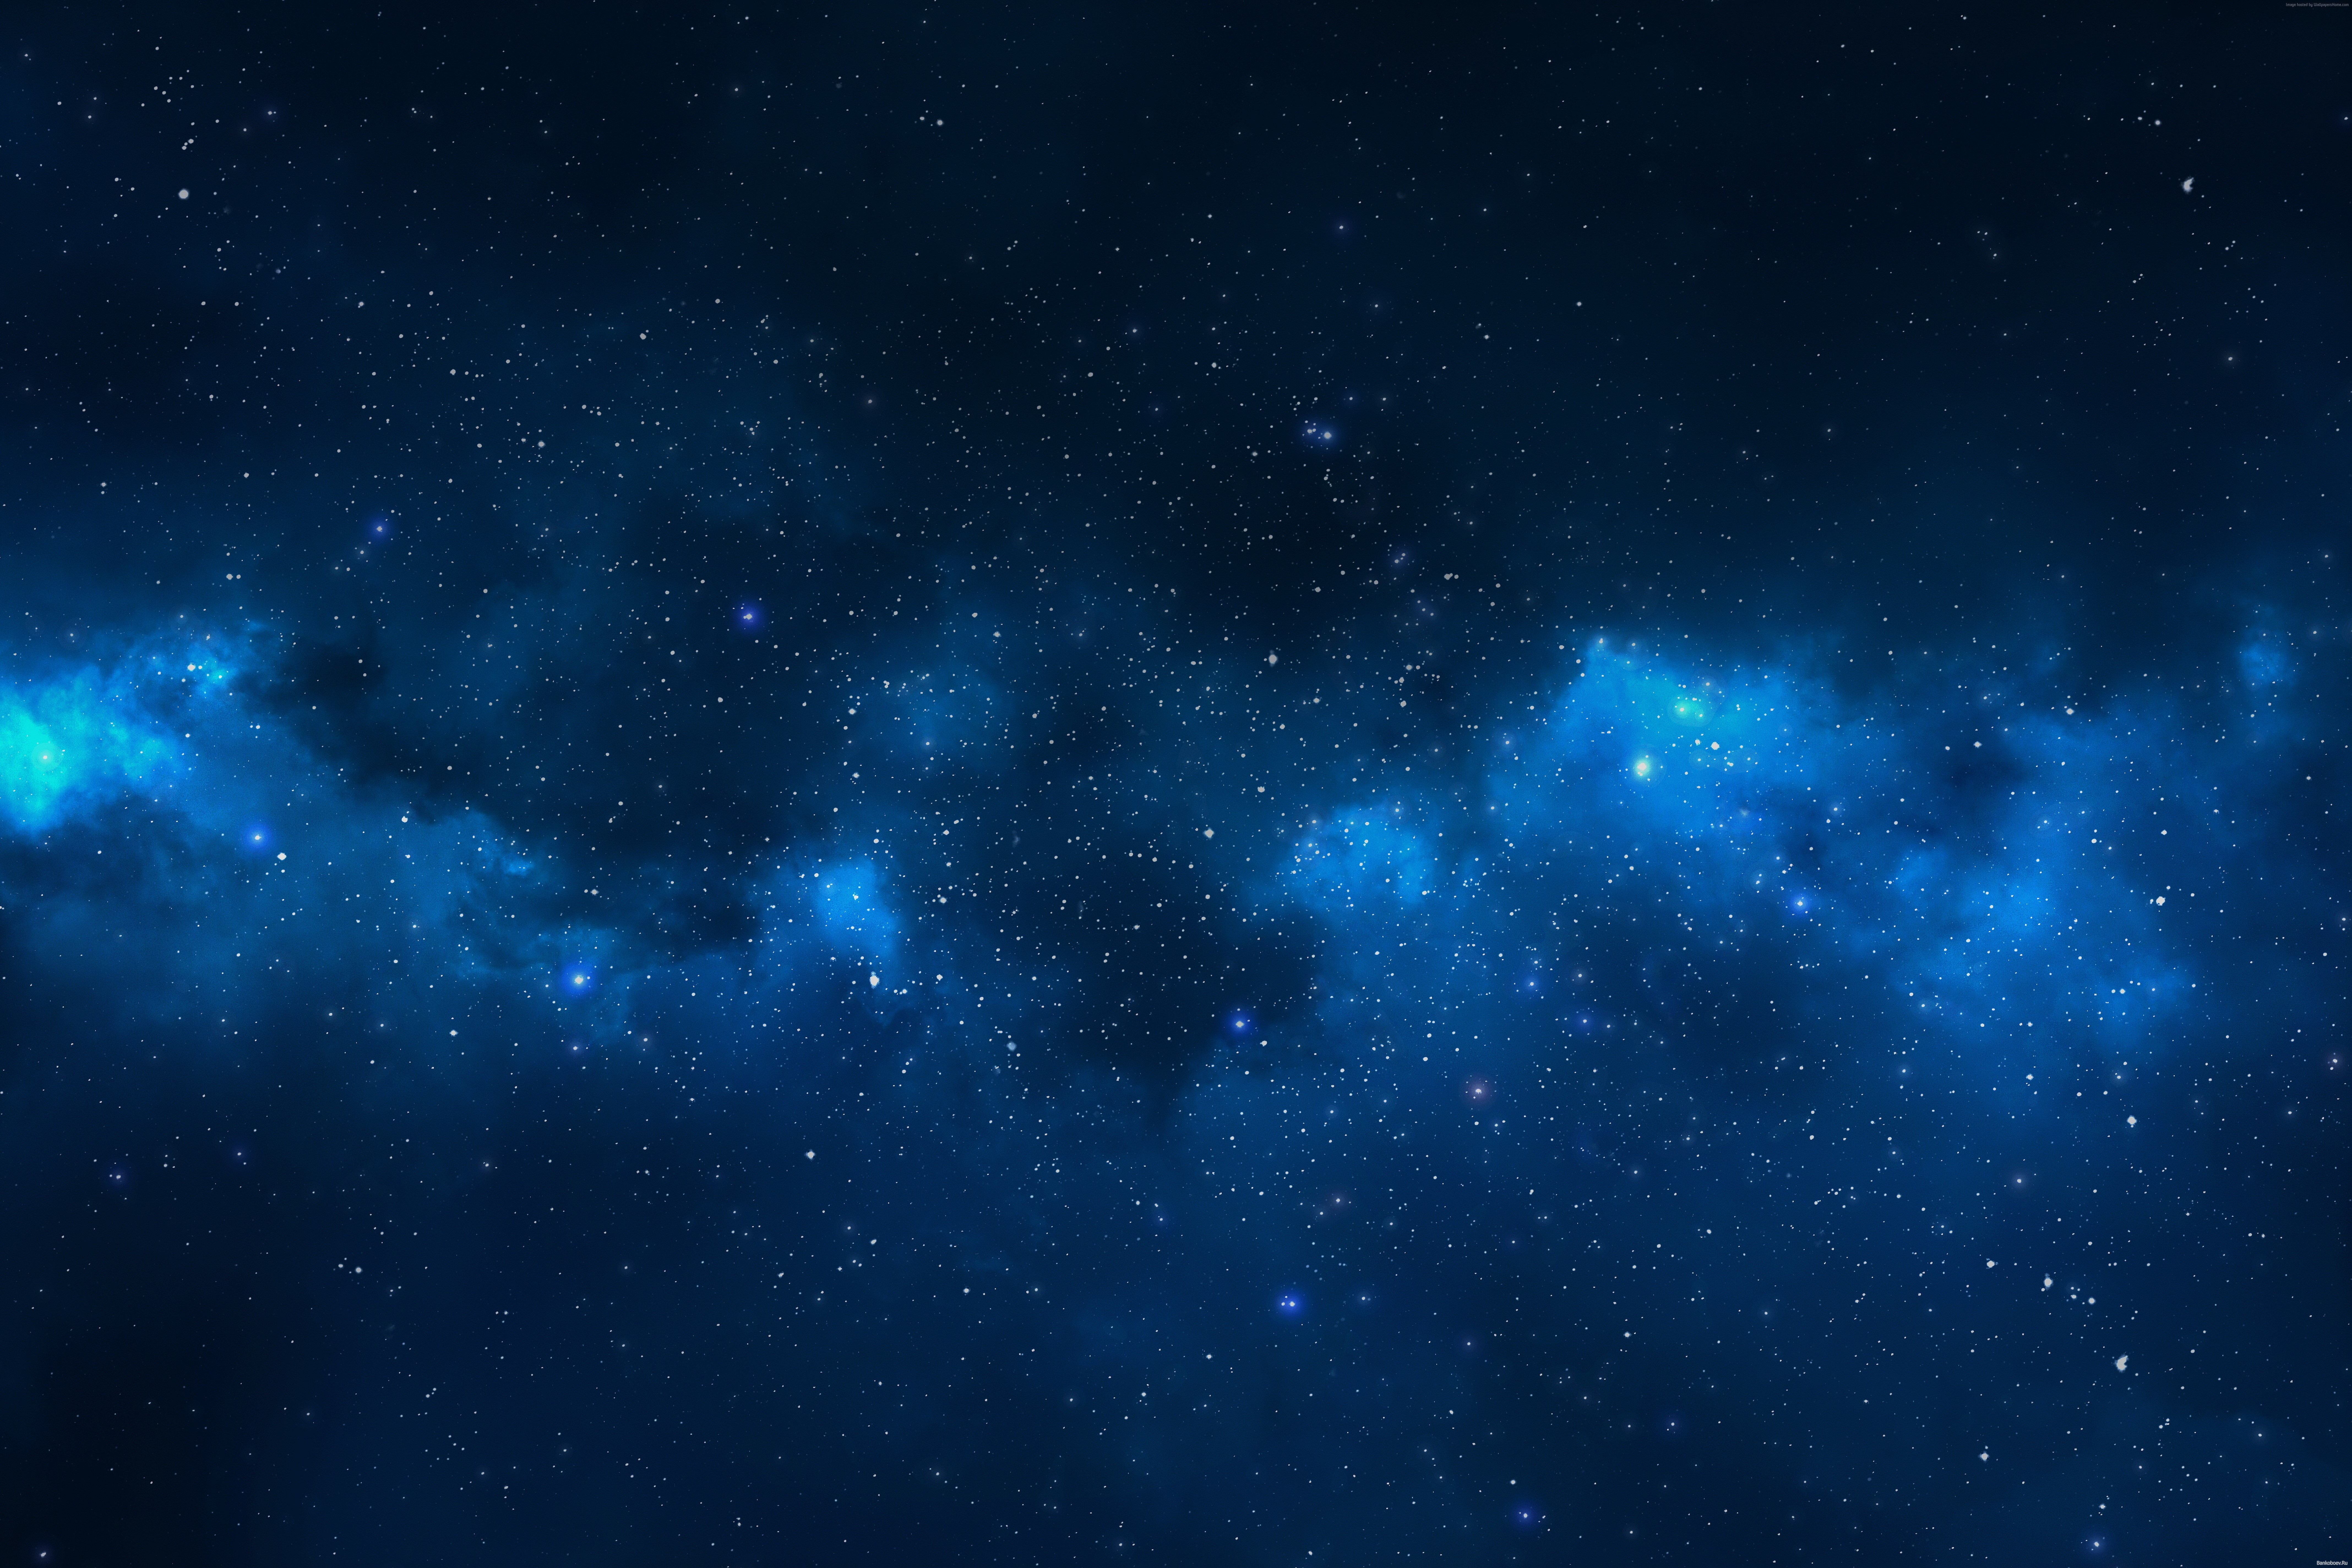
\includegraphics[scale=0.1855]{stars}}}
\centering
\vspace*{5cm}
\par\normalfont\fontsize{35}{35}\sffamily\selectfont
\textbf{Física del Magnetismo}\\
{\LARGE Notas de clase}\par
\vspace*{1cm}
%{\Huge Paolo Ricci, Ambrogio Fasoli}\par 
\endgroup
%--------------------------------------------------
\newpage
~\vfill
\thispagestyle{empty}

%\noindent Copyright \copyright\ 2014 Andrea Hidalgo\\ % Copyright notice
\noindent \textsc{Universidad Industrial de Santander \textbf{(UIS)} \\
Física Computacional en Materia Condensada  \textbf{(FICOMACO)}}\\
\url{http://www.uis.edu.co}\\

\noindent Profesor\\
Eduardo Alberto Orozco Ospino\\
eaorozco@uis.edu.co\\
\url{https://orcid.org/0000-0002-9884-9250}\\

\noindent Profesor\\
Andrés Camilo Garcia Castro\\
acgarcia@uis.edu.co\\
\url{https://orcid.org/0000-0003-3379-4495}\\

\noindent Estudiante\\
Juan Alejandro Pinto Castro\\
alejopintirris@gmail.com\\
\url{https://orcid.org/0000-0002-0937-4848}\\

\noindent \textsc{github.com/LaurethTeX/Clustering}\\ % URL

\noindent This research was done under the supervision of Dr. Pauline Barmby with the financial support of the MITACS Globalink Research Internship Award within a total of 12 weeks, from June 16th to September 5th of 2014.\\ % License information

\noindent \textit{Primera Edición, Diciembre 2018} % Printing/edition date
%--------------------------------------------------------------
\newpage
~\vfill
\thispagestyle{empty}
\noindent \begin{flushright}
\emph{"Los estudiantes que usan libros de texto de astrofísica siguen siendo esencialmente ignorantes de la propia existencia de los conceptos sobre el plasma, a pesar de que algunos de ellos se conocen desde hace medio siglo. La conclusión es que la astrofísica es demasiado importante para dejarla en manos de astrofísicos que han conseguido su conocimiento principal en estos libros de texto. Los datos de telescopios terrestres y en el espacio deben ser tratados por científicos que estén familiarizados con la física de laboratorio y de la magnetosfera, con la teoría de circuitos, y por supuesto con la moderna teoría del plasma.“\\
\vspace{3mm}
-Hannes Alfvén}
\end{flushright}

%http://www.frasesypensamientos.com.ar/autor/irving-langmuir.html
%---------------------------------------------------

\chapterimage{plasma_light_line_abstraction.jpg} % Table of contents heading image

\pagestyle{empty} % No headers
\renewcommand\contentsname{Contenido}
\tableofcontents % Print the table of contents itself

%\cleardoublepage % Forces the first chapter to start on an odd page so it's on the right

\pagestyle{fancy} % Print headers again


\chapterimage{boat.png}
\chapter{Magnetostática}

Campo físico (susceptible a ser medido) vectorial producido por cargas eléctricas en movimiento (corriente eléctrica) y que afectan cargas en movimiento.

\section{Preliminares}

En magnetostática, el campo magnético puede variar en el espacio, pero no en el tiempo.

\begin{itemize}
    \item $\vec{B}(\vec{r}) \longrightarrow$ Campo magnético estático producido por una distribución de corriente estacionaria.
    \item $\vec{J}(\vec{r})\longrightarrow$ Distribución de corriente estacionaria.
\end{itemize}{}

\subsection{Corriente Convencional vs Corriente Electrónica}

Es importante antes de entrar a deducir el concepto físico y matemático de corriente y densidad de corriente, aclarar una ambigüedad entre lo que se conoce como corriente convencional y corriente electrónica (real).

\begin{figure}[H]
\centering
\subfigure[]{\includegraphics[scale=0.45]{vel.png}}
\hspace{1cm}
\subfigure[]{\includegraphics[scale=0.45]{vele.png}}
\caption{(a) Corriente Convencional. (b) Corriente Electrónica.}
\label{Fig corriente}
\end{figure}

La \textbf{corriente convencional} se define como una corriente positiva de igual magnitud que la corriente real, es decir, el movimiento de los portadores de carga (q) van en dirección del campo externo, esto se muestra en la figura \ref{Fig corriente}(a). La \textbf{corriente electrónica o real} es la que en realidad ocurre físicamente, un campo eléctrico aplicado en un conductor en una dirección en específica (hacia la derecha en la figura (1.b)), hace que los electrones libres del medio se muevan en dirección opuesta al campo con velocidad de deriva $\vec{v_{d}}$, es por esto que el flujo de electrones o corriente electrónica va en dirección opuesta (negativa) al campo eléctrico aplicado.

\subsection{Corriente y Densidad de Corriente}

En la siguiente figura se ilustra una imagen ampliada de un tramo de un conductor lineal (alambre).

\begin{figure}[H]
\centering
\includegraphics[scale=0.5]{figdelta.png}
\caption{Alambre conductor}
\end{figure}

Definimos la distancia promedio recorrida por los portadores de cargas \textbf{móviles} y la concentración de portadores de cargas móviles como:

\begin{equation}  
    \Delta x\;=\;v_{d}\;{\Delta t} \quad ; \quad         n\;=\;\frac{N}{V}\;=\;\frac{\#  \text{partículas}}{\text{volumen}}
\label{Eq. 1}
\end{equation}

Donde $N$ es el número de cargas móviles y $V=A\;\Delta x$ es el volúmen en el cual se encuentran concentradas. Si conocemos la concentración $n$, conocemos el número de cargas $N$. Usando las ecuaciones de \ref{Eq. 1}, el número de portadores móviles que se encuentran en un tramo de longitud $\Delta x$ toma la forma:   

\begin{equation}
    N\;=\;n\;A\;v_{d}\;\Delta t
    \label{Eq. 3}
\end{equation}

Considerando la carga de los portadores móviles $q$, definimos la razón a la cual la carga neta  de los portadores móviles está contenida en $\Delta x$, es decir la carga neta que fluye a través de la sección transversal del alambre en un tiempo $\Delta t$.

\begin{equation}
    \Delta Q\;=\;q\;n\;V\;=\;q\;n\;A\;v_{d}\;\Delta t
    \label{Eq. 4}
\end{equation}

Definimos la corriente promedio como la razón a la cual la carga pasa en un tiempo $\Delta t$.
   
\begin{center}
\begin{large}
\begin{equation}
\tcboxmath[colback=white,colframe=gray, title=\centering Corriente eléctrica]
{I\;=\;\frac{\Delta Q}{\Delta t}\;=\;n\;q\;v_{d}\;A \qquad \left[\text{A}\;=\;\text{Ampere}\;=\;\frac{C}{s}\right]}  
\label{Eq. 5}
\end{equation}
\end{large}
\end{center}

Donde $I$ es la corriente (cantidad macroscópica), y $n,\;q,\;v_{d}$ son cantidades o propiedades microscópicas cuya magnitud caracterizan el flujo de los portadores. Vectorialmente la ecuación \ref{Eq. 5} se escribe como:

\begin{equation}
    I\;=\;n\;q\;\vec{v_{d}} \cdot \; \vec{A}  
\label{Eq. 6}
\end{equation}{}

Ahora podemos definir el vector de densidad de corriente como:

\begin{equation}
    \vec{J}\;=\;n\;q\;\vec{v_{d}}  \qquad \left[\frac{A}{m^2}\right]  \label{Eq. 7}
\end{equation}{}

Por lo tanto, si tenemos una densidad de corriente que es constante en el espacio y que la superficie a través de la cual la corriente fluye es plana, tenemos que la corriente se puede escribir como: 

\begin{equation}
    I\;=\;\vec{J} \cdot \vec{A}
    \label{Eq. 8}
\end{equation}

\section*{Generalización}

Si se tiene una distribución de corriente que no es constante (no homogénea) en el espacio, la expresión \ref{Eq. 8} ya deja de ser válida, al igual si la superficie de control deja de ser plana, por eso se requiere la generalización de la definición de la corriente y densidad de corriente para sistemas como el de la figura \ref{fig. sup}.

\begin{figure}[H]
\centering
\includegraphics[scale=0.5]{surf.png}
\caption{Caso general}
\label{fig. sup}
\end{figure}

Por lo tanto, la corriente que fluye a través de la superficie arbitraria S está dada por:

\vspace{-0.5cm}
\begin{center}
\begin{large}
\begin{equation}
\tcboxmath[colback=white,colframe=gray, title=\centering Corriente eléctrica generalizada]
{\mathrm{d}I=\vec{J} \cdot \mathrm{d} \vec{A} \quad \Longrightarrow \quad I= \int_{s} \vec{J}(\vec{r})\cdot \mathrm{d}\vec{A}  }  
\end{equation}
\end{large}
\end{center}

Donde $\vec{J}(\vec{r})\;=\;q\;n(\vec{r})\;\vec{v}(\vec{r})=\rho(\vec{r})\;n(\vec{r})$  y claramente, $\rho(\vec{r})$ es la densidad de carga eléctrica.

\section*{Caso General:}

En general, los sistemas eléctricos-magnéticos están formados por diferentes tipos de portadores de carga (electrones,iones unicargados o multicargados, etc.). Estos sistemas se les conoce como sistemas multiespecies donde $\alpha$ es el tipo de especie.

\begin{equation*}
    \vec{J}(\vec{r})=\sum_{\alpha}n_{\alpha}(\vec{r})q_{\alpha}v_{\alpha}(\vec{r})\quad \Longrightarrow \quad \vec{J}(\vec{r})=\sum_{\alpha}\rho_{\alpha}\vec{v}_{\alpha}(\vec{r})
\end{equation*}{}

\headrule

$$\vec{J}=n(-e)(-\mu_{E}\vec{E})=ne\mu_{E}\vec{E}$$. La conductividad eléctrica es entonces $\sigma=ne\mu_{E}\vec{E}$, que se relaciona con la resistividad eléctrica como $\rho=\frac{1}{\sigma}$. Teniendo en cuenta que el medio puede ser lineal o no lineal:

\begin{itemize}
    \item si $\sigma=\sigma(\vec{E}) \longrightarrow$ medio no lineal.
    \item si $\sigma\neq\sigma(\vec{E}) \longrightarrow$ no depende de $\vec{E}$, en un medio lineal $\vec{J} \propto\vec{E}$ (Ley de Ohm).
\end{itemize}

\begin{definition}
Medio anisotrópico:
\begin{equation*}
    J_{i}=\sigma_{ij}E_{j}
\end{equation*}
\end{definition}

\begin{minipage}[b]{0.5\textwidth}
\begin{definition}
Resistencia ($V_{2}-V_{1}>0$):
\begin{equation*}
    R=\frac{\Delta V}{I}=\frac{-\int_{P_{1}}^{P_{2}} \vec{E} \cdot \mathrm{d}\vec{l}}{\int_{s} \vec{J} \cdot \mathrm{d}\vec{A}}
\end{equation*}

Si $R=cte \Longrightarrow$ el material es óhmico.
\end{definition}
\end{minipage}
\begin{minipage}[b]{0.5\linewidth}
\begin{figure}[H]
    \centering
    \includegraphics[width=0.5\textwidth]{bitmap.png}
     \label{bitmap}
\end{figure}
\end{minipage}

\subsection*{¿Cómo calcular $R$?}

Consideremos que el campo eléctrico $\vec{E}$ es uniforme en todo el alambre, y despreciando efectos de borde, entonces.

\begin{equation}
\begin{split}
      \Delta V=V_{2}-V_{1}=-\int_{P_{1}}^{p_{2}} \vec{E}\cdot\mathrm{d}i&=-\int_{L}^{0} E_{x}\mathrm{d}x=E_{x}L\\
      I=\int\vec{J}\cdot\mathrm{d}\vec{A}=\sigma\int\vec{E}\cdot\mathrm{d}\vec{A}&=\sigma\int E_{x}\mathrm{d}A=\sigma E_{x}A\\
      R=\frac{\Delta V}{I}=\frac{E_{x}L}{\sigma E_{x}A} & \Longrightarrow R=\rho\frac{L}{A}
\end{split}
\end{equation}
 
\subsection{Ley de conservación de la carga eléctrica}

Vamos a calcular la corriente que fluye hacia la superficie usando la ecuación \ref{Eq. 8} y reescribiendo el diferencial:

\begin{equation*}
    I=\oint_{s} \vec{J}(\vec{r}) \cdot (-\hat{n}) \mathrm{d}A
\end{equation*}
 
Pero,

\begin{equation*}
    I=\frac{\mathrm{d}Q}{\mathrm{d}t} \quad ; \quad Q=\int_{V} \rho(\vec{r},t) \mathrm{d}^{3} r
\end{equation*}

Y teniendo en cuenta el teorema de la divergencia, tenemos que:

\begin{equation*}
    \frac{\mathrm{d}}{\mathrm{d}t}\int_{V} \rho(\vec{r},t) \mathrm{d}^{3}r=-\int_{V} \nabla\cdot\vec{J}(\vec{r},t) \mathrm{d}^{3}r \quad\Longrightarrow\quad
    \int_{V}\left[\frac{\partial\rho(\vec{r},t)}{\partial t}+\nabla\cdot\vec{J}(\vec{r},t)\right]\mathrm{d}^{3}r=0
  \end{equation*}

\begin{equation}
    \frac{\partial\rho(\vec{r},t)}{\partial t}+\nabla\cdot\vec{J}(\vec{r},t)=0
    \label{Eq. 1.10}
\end{equation}

La ecuación \ref{Eq. 1.10} representa la ecuación de continuidad de la carga eléctrica, entonces la \textbf{corriente estacionaria} se define a partir de esta ecuación. En una corriente estacionaria,

\begin{equation}
    \frac{\partial\rho(\vec{r},t)}{\partial t}=0\quad\Longrightarrow\quad \nabla\cdot\vec{J}(\vec{r})=0
    \label{Eq. 1.11}
\end{equation}

La ecuación \ref{Eq. 1.11} la podemos interpretar físicamente como la no existencia de fuentes ni sumideros de corrientes estacionarias. En su forma integral es:

\begin{equation*}
    \oint_{s}\nabla\cdot\vec{J}(\vec{r})\mathrm{d}s=\oint_{s}\vec{J}(\vec{r})\cdot\mathrm{d}\vec{A}=0
\end{equation*}

El campo eléctrico asociado a una corriente estacionaria se puede calcular por métodos electrostáticos debido a que no se ven afectadas las ecuaciones de la electrostática, ni la del potencial electrostático: $\nabla\cdot\vec{E}=0$, $\nabla\times\vec{E}=0$ y $\nabla^{2}\phi(\vec{r})=0$.

\begin{exercise}
Determine la resistencia entre las caras de los extremos de la arandela.

Partiendo de la ecuación de continuidad \ref{Eq. 1.10}, demuestre que en un conductor: $\rho(\vec{r},t)=\rho(\vec{r},t=0)e^{-\frac{\sigma}{\epsilon}t}$, donde $\tau=\frac{\epsilon}{\sigma}$ es la constante de relajación. Investigue el rango de validez del resultado con $\sigma=3\cdot 10^{-15}\left[\frac{s}{m}\right]$, $\epsilon_{r}=3$, entonces $\tau\leq 7.38[h]$.

\textbf{Rta:} $R=\frac{\pi}{2\sigma hl\frac{b}{a}}$
\end{exercise}


\section{Fundamentos de magnetostática en el vacío}

Las dos ecuaciones de la magnetostática en el vacío son:

\begin{equation}
    \nabla\cdot\vec{B}(\vec{r})=0\quad;\quad\nabla\times\vec{B}(\vec{r})=\mu_{0}\vec{J}(\vec{r})
    \label{Eq. 1.12}
\end{equation}

%\chapterimage{}
\chapter{De la clásica a la cuántica}
    \section{Origen de los momentos magnéticos}

El momento magnético en muchos libros lo denotas como $m_{z}$, pero la notación que se va a usar es $\vec{\mu}$. Usando la ley de Ampere en una corriente $I$ que circula en un anillo con un área $A$, tenemos que:

\begin{figure}[H]
\begin{minipage}[c]{0.5\linewidth}
    \centering
    \includegraphics[width=0.6\textwidth]{corriente.png}
    \caption{alambre conductor.}
    \label{Fig. 2.0}
    \end{minipage}
    \begin{minipage}[c]{0.5\linewidth}
\begin{equation}
    \mathrm{d}\vec{\mu}=I\mathrm{d}\vec{S}
    \label{Eq. 2.1}
\end{equation}
\end{minipage}
\end{figure}

Para encontrar el momento magnético total, se debe integrar la ecuación \ref{Eq. 2.1} sobre toda el área de la espira, entonces:

\begin{equation}
    \vec{\mu}=IA [Am]
\end{equation}

Cuando se habla de electricidad, hay lineas de campo que salen de las cargas positivas y líneas de campo que entran de las cargas negativas separadas por una distancia $l$ como se muestra en la figura \ref{Fig. 2.1}. El campo eléctrico va en dirección de las cargas negativas. La separación de cargas me genera un dipolo eléctrico $\vec{p}=l\cdot q$, esto es análogo en magnetismo al momento magnético.

\begin{equation*}
   \mu\Longrightarrow\vec{p}
\end{equation*}

\begin{figure}[H]
    \centering
    \includegraphics[width=0.9\textwidth]{electric-dipole.png}
    \caption{Campo electrostático $\vec{E}$ generado por un dipolo eléctrico en la dirección de la carga eléctrica negativa a una distancia $l$ de la carga eléctrica positiva. }
    \label{Fig. 2.1}
\end{figure}
\vspace{-7mm}

\begin{figure}[H]
\begin{minipage}[c]{0.6\linewidth}
\hspace{5mm} En magnetismo no existe el monopolo magnético como existe la carga, lo que existe es la separación de una carga que se esta moviendo en el tiempo en un anillo cerrado que encierra un área, voy a tener un momento magnético. en la imagen \ref{Fig. 2.0} se observa un anillo de dimensiones macroscópicas, es decir un fenómeno bastante grande. Ahora, en el mundo atómico lo que se esta moviendo en una trayectoria circular(simple) es el electrón, pero desde un punto de vista clásico, porque en realidad lo que esta pasando desde el punto de vista cuántico es que esa trayectoria circular son los orbitales del sistema. como se ilustra en la imagen \ref{Fig. 2.3}.
    \end{minipage}\hspace{5mm}
    \begin{minipage}[c]{0.4\linewidth}
    \centering
        \includegraphics[width=0.65\textwidth]{electron2.png}
    \caption{Representación del electrón\\ orbitando el núcleo atómico.}
    \label{Fig. 2.3}
\end{minipage}
\end{figure}
\vspace{-5.5mm}

El electrón se mueve super rápido, como tiene propiedades de carga y de masa, al tener el movimiento circular en el átomo, se tienen dos cosas: un $\vec{L}$ que es el momento angular relacionado con la masa, y un $\vec{\mu}$ que es el momento magnético relacionado con la carga. Si la masa se mueve orbitando el núcleo, entonces se tiene un momento angular. Si la carga se mueve tengo una corriente, entonces tengo un momento magnético.

Como el electrón tiene momento angular y momento magnético, existe una relación entre estos dos momentos.  Entre mas velocidad tiene el electrón, $\vec{L}$ va a ser mas grande y $\vec{\mu}$ mas grande. Los momentos están relacionados como:

\begin{equation}
    \vec{\mu}=\gamma\vec{L}
    \label{Eq. 2.3}
\end{equation}

Donde $\gamma$ es conocida como constante giromagnética. La relación \ref{Eq. 2.3} lleva a lo que se conoce como el efecto de Einstein-De Hass, que va ligado a la conservación del momento magnético angular en una barra solida de un sistema magnético.

\subsection{Energía}
La energía relacionada al momento magnético de un electrón inmerso en un campo magnético,

\begin{equation}
    E=-\vec{\mu}\cdot\vec{B}
    \label{Eq. 2.4}
\end{equation}

La ecuación \ref{Eq. 2.4} es análoga en electricidad a tener la energía eléctrica:

\begin{equation*}
    E=\vec{p}\cdot\vec{E}
\end{equation*}

La energía se va a minimizar en ambos casos, dependiendo de la dirección del campo. Con respecto al campo magnético, se va a tener una energía si el campo y el momento magnético son paralelos y otra energía si son antiparalelos. Dependiendo del fenómeno magnético, la energía se minimiza de forma paralela o antiparalela.

Los momentos magnéticos son susceptibles al torque magnético,

\begin{equation}
    \vec{G}=\vec{\mu}\times\vec{B}
    \label{Eq. 2.5}
\end{equation}

La ecuación \ref{Eq. 2.5} es análoga en electricidad al torque eléctrico:

\begin{equation*}
    \tau=\frac{\mathbf{d}\vec{L}}{\mathrm{d}t}=\vec{p}\times\vec{E}
\end{equation*}

Como el torque esta relacionado con el cambio del momento angular con respecto al tiempo, entonces si se deriva la ecuación \ref{Eq. 2.3} con respecto al tiempo, y usando la ecuación \ref{Eq. 2.5}, se tiene que:

\begin{equation}
    \frac{\mathrm{d}\vec{\mu}}{\mathrm{d}t}=\gamma\frac{\mathrm{d}\vec{L}}{\mathrm{d}t}=\gamma\vec{\mu}\times\vec{B}
    \label{Eq. 2.6}
\end{equation}

La ecuación \ref{Eq. 2.6} es de las primeras ecuaciones de la dinámica del momento angular desde la formulación clásica,.

\begin{example}
\begin{equation*}
      \vec{B}=B_{z}(E) \quad ;\quad \vec{\mu}=\mu_{x}\hat{i}+\mu_{y}\hat{j}+\mu_{z}\hat{k}
\end{equation*}

Aplicando las anteriores condiciones a la ecuación de precesión \ref{Eq. 2.6}:

\begin{equation*}
    \vec{\mu}\times\vec{B}=\begin{bmatrix}
    \hat{i} & \hat{j} & \hat{k} \\ 
    \mu_{x} & \mu_{y} & \mu_{z} \\ 
    0 & 0 & B_{z}
    \end{bmatrix}=\hat{i}(\mu_{y}B_{z})-\hat{j}(\vec{\mu_{x}}B_{z})
\end{equation*}

\begin{figure}[H]
\begin{minipage}[c]{0.6\linewidth}
\centering
        \includegraphics[width=0.5\textwidth]{momenmangetpng.png}
    \caption{Precesión del momento magnético del electrón en un campo magnético aplicado.}
    \label{Fig. 2.4}
    \end{minipage}\hspace{5mm}
    \begin{minipage}[c]{0.4\linewidth}
   \begin{equation*}
   \begin{split}
          \frac{\mathrm{d}\mu_{x}}{\mathrm{d}t}&=\gamma\mu_{y}B_{z}\\
          \frac{\mathrm{d}\mu_{y}}{\mathrm{d}t}&=\gamma\mu_{x}B_{z}\quad\\
          \frac{\mathrm{d}\mu_{z}}{\mathrm{d}t}&=0
   \end{split}
\end{equation*}
\end{minipage}
\end{figure}
\vspace{-4mm}

Lo que dicen las tres ecuaciones anteriores es que al aplicar un campo magnético, el momento magnético empieza a precesar con respecto al eje $z$, la componente en $z$ es constante, pero las componentes en $x$ y $y$ cambian en el tiempo. Resolviendo las tres ecuaciones diferenciales,

\begin{equation*}
        \mu_{x}(t)=\left|\vec{\mu}\right|sin(\theta)cos(\gamma Bt)\quad;\quad\mu_{y}(t)=\left|\vec{\mu}\right|sin(\theta)sin(\gamma Bt)\quad;\quad\mu_{z}(t)=\left|\vec{\mu}\right|cos(\theta)
\end{equation*}

Como el momento magnético está girando respecto a $z$, se forma una especie de cono, las componentes $x$ y $y$ van y vienen de forma sinusoidal sobre el cono dependiendo de una frecuencia $\omega_{L}=\gamma B$, conocida como la precesión de Larmor. Estas tres ecuaciones están incompletas porque no dicen que con el paso del tiempo el momento magnético va a empezar a converger en dirección al eje $z$, es decir va a girar sobre $z$ describiendo espirales cada vez mas pequeñas hasta perder el movimiento de precesión.
\end{example}

\subsection{El magnetón de Bohr}

La unidad básica para medir el momento magnético es el magnetón de Bohr. Se puede demostrar que cuando tengo un electrón con carga y masa, moviéndose alrededor del núcleo atómico, el momento angular orbital va en un sentido y el $\mu$ va en el otro (figura \ref{Fig. 2.5}),

\begin{figure}[H]
    \begin{minipage}[c]{0.4\linewidth}
        \begin{align*}
            A&=\pi r^{2}    &   \mu&=IA \\
            \vec{v}&=\frac{2\pi r}{T}   &   \vec{L}&=m_{e}\vec{v}r 
        \end{align*}
    \end{minipage}\hspace{2mm}
    \begin{minipage}[c]{0.6\linewidth}
        \centering
        \includegraphics[width=0.6\textwidth]{electron.png}
        \caption{Electrón orbitando el núcleo atómico.}
        \label{Fig. 2.5}
    \end{minipage}
\end{figure}
\vspace{-4mm}

Con las relaciones de las anteriores relaciones se puede llegar a la ecuación:

\begin{equation}
    \vec{\mu}=-\frac{e}{2m_{e}}\vec{L}
    \label{Eq. 2.7}
\end{equation}

La parte de $\frac{e}{2m_{e}}$ de la ecuación \ref{Eq. 2.7} tiene un parecido con la definición formal del magnetón de Bohr en el mundo cuántico.

\begin{equation}
    \mu_{B}\equiv\frac{e\hslash}{2m_{e}}
\label{Eq. 2.8}
\end{equation}

Pero la relación a la que se llega en la ecuación \ref{Eq. 2.7} viene de un formalismo de la mecánica clásica. Desde el punto de vista clásico queda incompleto cuando se va a medir. El magnetismo no se puede explicar completamente con mecánica clásica.

De la relación \ref{Eq. 2.7} se puede deducir la constante giromagnética y con esta la frecuencia de la precesión de Larmor: 

\begin{equation}
    \gamma=\frac{e}{2m_{e}} \quad ;\quad \omega_{L}=|\gamma|\vec{B}=\frac{e\vec{B}}{2m_{e}}
    \label{Eq. 2.9}
\end{equation}

Las relaciones de \ref{Eq. 2.9} vienen de una visión clásica.

\subsection{Magnetización}
La magnetización es una propiedad vectorial de la materia donde se suman los momentos magnéticos en total por unidad de volumen $\vec{M}:\frac{\mu}{v}$. Cuando se mide un material experimentalmente, no se mide el momento magnético, se mide la magnetización del sistema. El campo magnético es análogo al campo eléctrico en el vacío como:

\begin{equation}
    \vec{D}=\epsilon\vec{E}\quad\longrightarrow\quad\vec{B}=\mu_{0}\vec{H}
    \label{Eq. 2.10}
\end{equation}

Desde el punto de vista de electricidad, $\vec{D}$ es el vector de desplazamiento eléctrico, y en magnetismo pasa algo parecido, el vector $\vec{B}$ es conocido como inducción magnética con unidades de Tesla $[T]$ y el vector $\vec{H}$ es el campo magnético con unidades de $[\frac{A}{m}]$, que se relacionan con la constante de permeabilidad del espacio. Como estas ecuaciones están en el vacío, no hay ninguna molécula que sufra polarización o magnetización. Cuando tengo un material, entra a jugar la polarización y la magnetización , que es la respuesta del sistema al campo eléctrico y magnético, entonces la inducción magnética en \ref{Eq. 2.10} cambia debido a que el medios magnetiza:

\begin{equation}
    \vec{B}=\mu_{0}(\vec{H}+\vec{M})
    \label{Eq. 2.11}
\end{equation}

Si el material responde de una manera lineal al campo magnético aplicado, lo que sucede es que la magnetización va a aumentar como el campo magnético aplicado y es función lineal de las susceptibilidad magnética 

\begin{equation}
    \vec{M}=\chi\vec{H}
    \label{Eq. 2.12}
\end{equation}

Muy pocos materiales responden linealmente o algunos responden linealmente por un corto tiempo. Entonces:

\begin{equation}
    \vec{B}=\mu_{0}(1+\chi)\vec{H}=\mu_{0}\mu_{r}\vec{H}
    \label{Eq. 2.13}
\end{equation}

La ecuación \ref{Eq. 2.13} es análogo a $\vec{D}=\epsilon_{0}\epsilon_{r}\vec{E}$. Estos dos están entrelazados, cuando se acopla el magnetismo, se acopla la electricidad, entonces se tienen cargas que se mueven inmersas en campos magnéticos. 

\begin{remark}
Aveces se puede confundir entre quien es $\vec{B}$ y $\vec{H}$, incluso en artículos científicos. En electricidad es más claro, pero en magnetismo son indiferentes, aveces $\vec{B}$ es el campo aplicado, como aveces $\vec{H}$ es el campo aplicado. En algunos artículos científicos, para evitar el problema y cuando reportan una curva de histéresis lo que hacen es que colocan o $\vec{\mu_{0}}\vec{H}$, o $\vec{B}$.
\end{remark}

\section{Aproximación clásica}

Desde el punto de vista de la aproximación clásica del magnetismo tenemos que la única fuente de tener campo magnético o momento magnético es una carga que se mueve, puede estar orbitando alrededor del núcleo de manera clásica que no puede saltar entre orbitales de manera cuántica porque no estoy teniendo en cuenta energía cuantizada. La única fuente de magnetismo va a ser el momento magnético orbital. Existe una partícula que va a estar inmersa en un campo magnético y un campo eléctrico que se describe mediante la fuerza de Lorentz clásica:

\begin{equation}
    \vec{F}=q\left(\vec{E+v\times\vec{B}}\right)
    \label{Eq. 2.14}
\end{equation}

Describiendo la fuerza y los campos de manera:

\begin{equation}
    \vec{F}=\frac{\mathrm{d}\vec{v}}{\mathrm{d}t}\quad;\quad\vec{B}=\nabla\cdot\vec{A}\quad;\quad\nabla V=\vec{E}+\frac{\partial\vec{A}}{\partial t}
    \label{Eq. 2.15}
\end{equation}

Donde $\vec{v}$ es la velocidad de la partícula y $\vec{A}$ es un potencial vectorial magnético. Si se mezclan las ecuaciones \ref{Eq. 2.13} y \ref{Eq. 2.14} se va a obtener una ecuación diferencial de movimiento para la partícula que va a ser:

\begin{equation}
    \frac{\mathrm{d}\vec{v}}{\mathrm{d}t}=-q\nabla V-q\frac{\partial\vec{A}}{\partial t}+q\vec{V}\times\left(\nabla\times\vec{A}\right)
    \label{Eq. 2.16}
\end{equation}

Usando la identidad vectorial del triple producto cruz y la derivada total

\begin{equation*}
    \vec{v}\times\left(\nabla\times\vec{A}\right)=\nabla\left(\vec{v}\cdot\vec{A}\right)-\left(\vec{v}\cdot\nabla\right)\vec{A}\quad;\quad\frac{\mathrm{d}}{\mathrm{d}t}=\frac{\partial}{\partial t}+\frac{\partial\vec{r}}{\partial t}\frac{\partial}{\partial\vec{r}}
\end{equation*}

obtenemos:

\begin{equation}
\frac{\mathrm{d}}{\mathrm{d}t}\left(m\vec{v}+q\vec{A}\right)=q\nabla\left(V-\vec{v}\cdot\vec{A}\right)    
\label{Eq. 2.17}
\end{equation}

El término de la izquierda de la igualdad de \ref{Eq. 2.17} es básicamente un momento de la partícula y se le conoce como momento canónico. Lo que se ve en esta ecuación es que el efecto del campo magnético en las ecuaciones no va a quedar implícito, va a quedar a través del potencial vectorial y en función del momento de las partículas, se va a obtener una ecuación diferencial que depende del momento de las partículas, y ese momento de las partículas se va a ver afectadas por el campo eléctrico, pero en la ecuación \ref{Eq. 2.17}, se ven los campos a través de los potenciales. si se quiere saber la energía cinética de la partícula, se puede despejar la velocidad en $K=\frac{1}{2}mv^{2}$, entonces dentro del punto de vista vectorial la energía cinética de la partícula es:

\begin{equation}
    K=\frac{1}{2m}\left(\vec{P}+q\vec{A}\right)^{2}
    \label{Eq. 2.18}
\end{equation}

La partícula va a estar sometida a $\vec{v}$ y a $\vec{A}$. En mecánica cuántica la ecuación \ref{Eq. 2.18} es llamado operador energía cinética:

\begin{equation}
    \hat{K}=\left(-i\hslash\nabla+q\vec{A}\right)^{2}\cdot\frac{1}{2m}
    \label{Eq. 2.19}
\end{equation}

El teorema de Bohr-van Leeuwen dice que se puede hacer todo el anterior desarrollo teniendo en cuenta la mecánica estadística. Un montón de partículas forman un ensamble y una cantidad de estados posibles, esas partículas pueden tener una distribución que va a través de una función de partición. Desde el punto de vista clásico la magnetización tiene que ser función del campo magnético aplicado, entonces si hay campo magnético aplicado no hay magnetización. La función de partición va a ser una función que suma sobre todas las partículas del sistema (material), como los momentos magnéticos están en diferentes direcciónes, se suman sobre todo el sólido, entonces se debe tener en cuenta la posición y el momento de forma vectorial así que la integral es de tantas dimensiones sobre cada un de las $N$ partículas y suma sobre la posición y el momento de cada partícula. En ausencia de campo, el potencial vectorial es cero, entonces todas hacen movimientos aleatorios, en total da cero.

\begin{figure}[H]
    \centering
    \includegraphics[width=0.4\textwidth]{material.png}
    \caption{electrones del sólidos desde un punto de vista clásico formando trayectorias circulares.}
    \label{Fig. 2.6}
\end{figure}

Suponiendo que se logra aplicar el campo magnético, va a ver en el promedio de todo el sólido algo parecido a la figura \ref{Fig. 2.6}, en la superficie todos van a querer girar en el mismo sentido, pero ya no pueden terminar la trayectoria. Los momento magnético en el centro del sólido van en dirección fuera del plano. En la superficie los electrones brincan y generan una corriente en dirección de las manecillas del reloj, pero en el centro se genera una corriente en contra de la dirección de las manecillas del reloj. Al fina la magnetización va a ser cero.

Si no se hace uso de la mecánica cuántica y de la teoría del espín, que es un momento adicional, no se podrá entender la magnetización. Una de las cosas que no puede explicar la mecánica clásica es la magnetización en un sólido en ausencia de campo magnético. La magnetita es un oxido de hierro que tiene momento magnético sin haber sido sometida a campo magnético.

\section{Aproximación cuántica}

El momento angular sigue siendo $\vec{L}$ que depende de un electrón que esta orbitando, pero desde el punto de vista de la aproximación cuántica es mas complejo por tener estados cuantizados de energía. Como se puede tener varios orbitales en un átomo hidrogenoide, entonces $\vec{L}$ va a depender del orbital en el que este porque el electrón puede brincar entre orbitales. En mecánica cuántica se divide $\vec{L}$ en dos: 

\begin{figure}[H]
    \begin{minipage}[c]{0.4\linewidth}
       \begin{itemize}
           \item El momento angular orbital $\vec{\hat{L}}$ con valores propios $\sqrt{l(l+1)}\hslash$.
            \item La proyección sobre $z$ del momento angular orbital $\hat{\vec{L}}_{z}$ con valores propios $m_{l}\hslash$.
      \end{itemize}
    \end{minipage}\hspace{2mm}
    \begin{minipage}[c]{0.6\linewidth}
        \centering
        \includegraphics[width=0.5\textwidth]{l2lz2.png}
        \caption{Operadores momento angular orbital $\vec{\hat{L}}$ y $\hat{\vec{L}}_{z}$ .}
        \label{Fig. 2.7}
    \end{minipage}
\end{figure}
\vspace{-4mm}

Para que el $\hat{\vec{L}}$ este en la dirección como esta en la imagen \ref{Fig. 2.7} tendría que estar orbitando perpendicularmente, pero esa trayectoria depende del orbital. $\hat{\vec{L}}$ depende del orbital, entonces siempre por simetría se toma un operador $\hat{\vec{L}_{z}}$ como eje de referencia debido a que como el electrón va a estar en cualquier orbital, es mucho mas complejo saber donde está. Siempre se debe tener un eje de referencia de simetría de toda la mecánica cuántica del sistema. El momento angular se puede relacionar con el momento magnético del sistema por la ecuación \ref{Eq. 2.3}. Ahora para magnetismo se tienen dos operadores:

\begin{itemize}
    \item Operador magnético $\hat{\vec{\mu}}$ con valores propios $\sqrt{l(l+1)}\mu_{B}$, este operador está relacionado con los estados de momento angular orbital $\hat{\vec{L}}$.
    \item Proyección del operador magnético en $z$ $\hat{\vec{\mu}_{z}}$ con valores propios $-m_{l}\mu_{B}$.
\end{itemize}

El momento angular orbital $\vec{L}$ del sistema ahora es un momento angular orbital cuántico $\hat{\vec{L}}$. Los valores propios de $\hat{\vec{\mu}_{z}}$ son negativos porque ele momento angular orbital va  en un sentido pero el momento magnético va en el sentido contrario. Las partículas que en este caso son electrones, tienen un momento angular intrínseco llamado espín. Es"como si" el electrón girara sobre su propio eje, pero esto no es así, solamente es una analogía ara la parte clásica. Ese momento intrínseco esta ligada a la rotación de la partícula sobre su eje, entonces por ser partícula cargada tiene momento magnético. Hay que hacer énfasis en que el último argumento es solo para dar a entender la idea.

\subsection{Espín}

El espín es un momento magnético angular intrínseco del electrón, explica más a detalle el magnetismo y cantidad de fenómenos cuánticos en física. Conectar la parte clásica con la pare cuántica es importante, en el caso de magnetismo el espín del electrón juega la parte importante de esto porque por simetría del orbital, es decir por los números cuánticos del sistema, $l$ puede ser cero, en total $\hat{\vec{L}}$ es cero o muy pequeño, entonces $\vec{\mu}$ relacionado con $\hat{\vec{\mu}}$ es muy pequeño. El responsable del magnetismo en un sistema es el espín. Se puede desglosar  el magnetismo en un sistema en contribuciones de orbital o de espín.

El espín es otro número cuántico $\vec{S}$ con valores $\pm\frac{1}{2}$, número cuántico $s$ con número de estados accesibles $(2s+1)$. Para el electrón se tienen dos estados posibles $+\frac{\hslash}{2}$ y $-\frac{\hslash}{2}$. Como es un sólido, la naturaleza magnética se debe a los electrones en gran parte. 

\begin{equation*}
    \hat{\vec{S}}\longrightarrow s(s+1)\hslash\quad;\quad s_{z}=m_{s}\hslash
\end{equation*}

Siempre en un sistema cuántico se tiene un eje sobre el cuál se tiene la magnetización y otro que va a ser la proyección. El momento magnético que viene del espín $m$ por notación, entonces:

\begin{equation}
        m_{z}=-g\mu_{B}m_{s}\quad;\quad        m=\sqrt{s(s+1)}g\mu_{B}\equiv\frac{\sqrt{3}}{2}g\mu_{B}
\label{Eq. 2.20}
\end{equation}

Donde $g$ es conocido como el factor de Landé, el cual es una proporcionalidad entre el momento magnético y el magnetón de Bohr. Si el sistema es perfecto $g$ tiene un valor de dos, quiere decir que si es perfecto, el momento magnético en $z$ es aproximadamente el momento magnético de un electrón. Por principio de exclusión de Pauli cuando se logra definir ele espín a lo largo de un eje, el sistema no se puede definir en los otros dos ejes. En la imagen \ref{Fig. 2.8} se puede ver la relación entre el momento del espín con el momento total del espín. 

\begin{remark}
El momento magnético $\vec{\mu}$ viene del orbital, mientras que $\vec{m}$ viene del espín.
\end{remark}

\subsection{Energía del efecto Zeeman}

Hay una energía asociada cuando  se tiene campo magnético asociado. El electrón puede estar en dos estados $+\frac{1}{2}$ y $-\frac{1}{2}$ que son estados degenerados porque la proyección no se ha decidido. El efecto que tiene el campo magnético aplicado a un sistema cuando se tiene en cuneta el espín es conocido como efecto Zeeman o en inglés 'Zeeman splitting' (figura \ref{Fig. 2.8}). El campo magnético rompe la degeneración de los estados de espín permitidos en el sistema y hace que se colapse uno de los dos estado del sistema. La energía de Zeeman se expresa como:

\begin{equation}
            E_{z}=g\mu_{B}m_{s}B
            \label{2.21}
\end{equation}

\begin{figure}[H]
        \centering
        \includegraphics[width=0.6\textwidth]{splitting.png}
        \includegraphics[width=0.3\textwidth]{splitting-cart.png}
        \caption{(a) División de la energía debido al campo magnético aplicado (efecto Zeeman). (b) Operadores $\hat{\vec{S}}$ y $\hat{\vec{S}}_{z}$ en el pano cartesiano.}
        \label{Fig. 2.8}
\end{figure}

Cuando $B=0\longrightarrow E_{z}=0$, cuando $B=B_{0}$ entonces la energía de Zeeman tiene dos energías posibles: $E_{z}=+\mu_{B}B$ y $E_{z}=-\mu_{B}B$. Los estados degenerados del electrón se dividen en dos. En un sistema se parte la degeneración del espín aplicando un campo magnético. El salto de energía equivale entonces a $2\mu_{B}B$ que va ligado con la intensidad del campo magnético. En un material real $g$ depende de como $\hat{\vec{L}}$ y $\hat{\vec{S}}$ se acoplan.

Para poder abordar el magnetismo podemos conocer las ecuaciones de Maxwell pero no son suficientes en explicar muchos fenómenos con el de magnetismo en ausencia de campo magnético. Magnetismo es puramente cuántico, el espín va ligado a un momento magnético de la partícula.

\subsection{Matrices de Pauli}

Surgen de tratar de entender como es la proyección y como funcionan los espines y mapear los estados accesibles e inaccesibles. El momento magnético intrínseco de la partícula no va ligado a ningún giro. Si el espín fuese un vector, tiene que tener una orientación en el espacio, pero como se define esa orientación en el espacio. Las matrices de Pauli condensa la información de estados accesible.

Encontrar un  estado para una partícula que puede tener dos estados posibles en base a una partícula simple con espín. Se usará la notación de Dirac en estos dos estados. El espín y por ende la magnetización no son vectores, son pseudo vectores, entonces el espín no es invariante bajo ciertas transformaciones realizadas a un tensor asociado con el espín. Desde el punto de vista tensorial, si se aplica una transformación a un vector, este es invariante ante esta transformación, pero el espín varía con la transformación porque ese cambio le agrega un signo menos. A los estados del espín se les asigna un tensor:

\begin{equation}
    \ket{\uparrow}=\binom{1}{0} \qquad;\qquad \ket{\downarrow}=\binom{0}{1}
    \label{Eq. 2.22}
\end{equation}

Entonces, por \ref{Eq. 2.22} cuando se quiere encontrar el estado combinado de esos dos espines asumimos que esos dos espines pueden existir en un mismo sistema,

\begin{equation}
\ket{\upuparrows}=\ket{\uparrow}\ket{\uparrow}=a_{i}b_{j}=c_{ij}=\begin{pmatrix}
1 & 0 \\ 
0 & 0
\end{pmatrix} 
\label{Eq. 2.23}
\end{equation}

Se encuentra quien es el estado en base al álgebra tensorial porque aunque el espín no sea un vector lo puedo expresar como un tensor.

\begin{example}
Puedo tener cantidades físicas que actúan como tensores pero no son vectores o matrices.
El estrés es un caso clásico que actúa como tensor pero no es un vector.
\end{example}

Calculando los demás estados igual que se calculó la ecuación \ref{Eq. 2.23},

\begin{equation}
    \ket{\downdownarrows}=\begin{pmatrix}
                            0 & 0 \\ 
                            0 & 1
\end{pmatrix} \qquad;\qquad\ket{\downdownarrows}=\begin{pmatrix}
                                                    0 & 0 \\ 
                                                    0 & 1
\end{pmatrix} \qquad;\qquad\ket{\uparrow\downarrow}=\begin{pmatrix}
                                                    0 & 1 \\ 
                                                    0 & 0
\end{pmatrix} \qquad;\qquad\ket{\downarrow\uparrow}=\begin{pmatrix}
                                                    0 & 0 \\ 
                                                    1 & 0
\end{pmatrix} 
\label{Eq. 2.24}
\end{equation}

Las ecuaciones \ref{Eq. 2.23} y \ref{Eq. 2.24} son estados individuales, al combinar los estados del sistema, se toman las combinaciones lineales,

\begin{equation}
\begin{split}
    \frac{1}{\sqrt{2}}\left[\ket{\uparrow\downarrow}+\ket{\downarrow\uparrow}\right]=\frac{1}{\sqrt{2}}\begin{pmatrix}
                0 & 1 \\
                1 & 0
    \end{pmatrix}= \frac{1}{\sqrt{2}}\sigma_{1}=\sigma_{x}\\
    \frac{1}{\sqrt{2}}\left[\ket{\uparrow\downarrow}-\ket{\downarrow\uparrow}\right]=\frac{1}{\sqrt{2}}\begin{pmatrix}
                0 & 1 \\
                -1 & 0
    \end{pmatrix}= -\frac{i}{\sqrt{2}}\sigma_{2}=\sigma_{y}\\
    \frac{1}{\sqrt{2}}\left[\ket{\uparrow\uparrow}-\ket{\downarrow\downarrow}\right]=\frac{1}{\sqrt{2}}\begin{pmatrix}
                1 & 0 \\
                0 & -1
    \end{pmatrix}= \frac{1}{\sqrt{2}}\sigma_{3}=\sigma_{z}
\end{split}
\label{Eq. 2.25}
\end{equation}

En la ecuación \ref{Eq. 2.25} están contenidas las matrices de Pauli, $\sigma_{z}$ es diagonal porque implícitamente se escogió el sistema orientado o proyectado en base a un eje de simetría o referencia el cual es $z$ y sale de combinar todos los estados $\ket{\upuparrows}$ con todos los estados $\ket{\downdownarrows}$. Adicionalmente traen información relativamente compleja porque no es solo decir cual esta up y cual down pero en cualquier parte del espacio. Es como decir que va a ocupar un estado que se asume  como una partícula girando sobre su propio eje pero que en realidad son dos estados que se denominan 'up' o 'down' que usualmente se toma un eje de simetría que es $z$ para proyectar el estado y ver que es lo que pasa en el sistema, lo que no se puede hacer con $\sigma_{x}$ y $\sigma_{y}$ porque contiene términos fuera de la diagonal.

\begin{exercise}
Si la partícula se midiera y la medición del espín resulta en $x$, ¿se puede medir es $y$?\\

\textbf{R:} No, porque además de que la matriz de Pauli $\sigma_{y}$ es compleja, no conmutan. Es decir si se hace un experimento y se mide primero en $x$, luego en $y$, el resultado es diferente si se hace primero en $y$ y luego en $x$.
\end{exercise}

\begin{remark}
Muchas de las cosas que se ven en mecánica cuántica son complejas porque no se pueden ver solo hasta que se proyectan. Las funciónes de onda son un ente matemático, cuando se quiere encontrar la función de onda, se hace $\braket{\phi}$ y automáticamente se va el $i$ y se puede observar la intensidad, lo que es una cantidad al cuadrado. El espín se le está agregando a las funciónes de onda que podrán distinguir entre espín 'up' y espín 'down'.
\end{remark}

\subsection{Operador de espín}

El operador $\hat{\vec{\sigma}}$ tiene componentes $\hat{\vec{\sigma}}=(\hat{\vec{\sigma}}_{x},\hat{\vec{\sigma}}_{y},\hat{\vec{\sigma}}_{z})$. Decir que el espín está proyectado sobre una de las direcciónes es una sobre-simplificación porque es algo más complejo. En realidad el operador $\hat{\vec{\sigma}}$ es como una vector de matrices que cuando se coloca en la ecuación de Schrödinger se convierte en la ecuación de Dirac. El operador de espín viene de las matrices de Pauli $\hat{\vec{S}}=\frac{1}{2}\hat{\vec{\sigma}}$, como cada operador resulta en un observable, se tiene que definir en que estado esta y definirlo a lo largo de un eje y por ende se tiene incertidumbre en otro eje.

\begin{equation}
    \hat{\vec{S}}_{x}=\frac{1}{2}\begin{pmatrix}
                                    0 & 1 \\
                                    1 & 0 
                               \end{pmatrix}\qquad;\qquad\hat{\vec{S}}_{y}=\frac{1}{2}\begin{pmatrix}
                                    0 & -i \\
                                    i & 0 
                               \end{pmatrix}\qquad;\qquad\hat{\vec{S}}_{z}=\frac{1}{2}\begin{pmatrix}
                                    1 & 0 \\
                                    0 & -1 
                               \end{pmatrix}\qquad;\qquad
    \label{Eq. 2.26}                            
\end{equation}

En algunos libro tienen en cuenta $\hslash$, n otros no, pero el momento angular asociado al espín va a estar ligado a $\hat{\vec{S}}=\frac{\hslash}{2}\hat{\vec{\sigma}}$, entonces se pueden tener dos estados:

\begin{equation}
    \ket{\uparrow_{z}}=\binom{1}{0}\quad;\quad\ket{\downarrow_{z}}=\binom{0}{1}
    \label{Eq. 2.27}
\end{equation}

Si se aplica la ecuación \ref{Eq. 2.27} a una ecuación de valores y vectores propios,

\begin{equation}
    \hat{\vec{S}}_{z}\ket{\uparrow_{z}}=\frac{1}{2}\ket{\uparrow_{z}}\quad;\quad\hat{\vec{S}}_{z}\ket{\downarrow_{z}}=-\frac{1}{2}\ket{\downarrow_{z}}
    \label{Eq. 2.28}
\end{equation}

en las ecuaciones \ref{Eq. 2.28} el valor esperado del operador es $\frac{1}{2}$ y $-\frac{1}{2}$, respectivamente. Ahora para el caso del eje $x$:

\begin{equation}
    \ket{\uparrow_{x}}=\binom{1}{1}\quad;\quad\ket{\downarrow_{x}}=\binom{1}{-1}
    \label{Eq. 2.29}
\end{equation}

La ecuación \ref{Eq. 2.29} esta normalizada y tiene este resultado porque no se puede diagonalizar. Ahora con respecto al eje $y$:

\begin{equation}
    \ket{\uparrow_{y}}=\binom{1}{i}\quad;\quad\ket{\downarrow_{y}}=\binom{1}{-i}
    \label{Eq. 2.30}
\end{equation}

Las ecuaciones \ref{Eq. 2.27}, \ref{Eq. 2.29} y \ref{Eq. 2.30} funciónan para entender como entra el magnetismo en la materia condensada y en mecánica cuántico y entra a través de espínores.

\subsection{espínores}

En mecánica cuántica el espín tiene un momento magnético de espín asociado. La función de onda que ya se conoce se acopla con el espín, es lo que se conoce como espínor. Un material con electrones va a tener magnetismo, la función de onda hay que agregarle el espín. La función de onda incluyendo los espínores,

\begin{equation*}
    \ket{\psi}=\binom{a}{b}\equiv a\ket{\uparrow_{z}}+b\ket{\downarrow_{z}}\quad;\quad ab\quad\text{Números complejos}
\end{equation*}

Como debe estar normalizada, entonces $a^{2}+b^{2}=1$. El operador de espín proyectado en las coordenadas cartesianas es:

\begin{equation}
    \hat{\vec{S}}=\begin{pmatrix}
                    \hat{S}_{x}\\
                    \hat{S}_{y}\\
                    \hat{S}_{z}
                \end{pmatrix}\equiv\hat{i}\hat{S}_{x}+\hat{j}\hat{S}_{y}+\hat{S}_{z}
    \label{Eq. 2.31}
\end{equation}

La ecuación \ref{Eq. 2.31} conlleva a:

\begin{equation}
    \hat{\vec{S}}^{2}=\hat{S}_{x}^{2}+\hat{S}_{y}^{2}+\hat{S}_{z}^{2}
    \label{Eq. 2.32}
\end{equation}

Cuando se tiene un operador que no esta a lo largo de $z$, se dice que no están diagonalizado, pero para cualquiera de los tres operadores componente del operador de \ref{Eq. 2.32} los autovalores son $\pm\frac{1}{2}$.

\begin{example} Los operadores de espín no conmutan. 

\begin{equation*}
    \left[\hat{S}_{x},\hat{S}_{y}\right]=i\hat{S}_{z}
\end{equation*}

Pero hay un operador que si conmuta

\begin{equation*}
    \left[\hat{S}^{2},\hat{S}_{z}\right]=0
\end{equation*}

debido a que $\hat{S}^{2}$ incluye todos tos operadores componente de la ecuación \ref{Eq. 2.32}, es como tener una esfera y luego conmutarlo con el eje principal de la esfera.

\end{example}

En el plano las matrices de Pauli no son diagonales y en $y$ es un eje complejo, entonces el plano es en realidad es el plano de Argand. Cuando el espín esta totalmente resuelto en $z$ la matriz es diagonal y es perpendicular al plano complejo, pero si no esta totalmente definido en $z$, se tiene una proyección en el espacio complejo.
%%%imange minipage

\begin{equation*}
    \vec{S}=\frac{1}{\sqrt{1+|q|^{2}}}\binom{1}{q}
\end{equation*}

Si el el espín tiene componente $z$ y plano complejo, siempre el espín va a ser $1$ y $q$ donde $q$ es el plano complejo.

\subsection{Operadores escalera}

Se construyen estados accesibles con los operadores de subida y de bajada:

\begin{equation}
    \hat{S}_{+}=\hat{S}_{x}+i\hat{S}_{y}\quad;\quad\hat{S}_{-}=\hat{S}_{x}-i\hat{S}_{y}
    \label{Eq. 2.33}
\end{equation}

Se puede subir y bajar de estados a través de las ecuaciones de \ref{Eq. 2.33}. Lo que dicen estas ecuaciones es que estos operadores son no Hermitianos ($\hat{A}^{\dagger}\neq\hat{A}$) debido a que como no es invariante ante transformaciones el adjunto conjugado (operador daga) no es el mismo, es decir,

\begin{equation}
    \hat{S}_{+}^{\dagger}=\hat{S}_{-}\quad;\quad\hat{S}_{-}^{\dagger}=\hat{S}_{+}
    \label{Eq. 2.34}
\end{equation}

Se esta brincando entre espines, La ecuación \ref{Eq. 2.34} lo que se hace es rotar e invertirlo, aunque no lo podemos entender como rotaciones, sigue teniendo esa cuestión de simetría. 
Volviendo a los conmutadores, tenemos:

\begin{equation*}
    \begin{split}
        \left[\hat{S}_{+},\hat{S}_{-}\right]=2\hat{S}_{z}\\
        \left[\hat{S}_{z},\hat{S}_{\pm}\right]=\pm\hat{S}_{\pm}\\
        \left[\hat{S}^{2},\hat{S}_{\pm}\right]=0\\
    \end{split}
\end{equation*}

$hat{S}_{+} y \hat{S}_{-}$ son los operadores de subida y de bajada. En todo el sólido se tiene $\hat{S}^{2}$, cuando vamos a encontrar quien es este operador, es la ecuación \ref{Eq. 2.32}, cuando se usa esta ecuación con los conmutadores antes mencionados, entonces podemos definir el operador $\hat{S}^{2}$ en función del operador $z$ y los operadores de subida y de bajada.

\begin{equation}
    \hat{S}^{2}=\frac{1}{2}\left(\hat{S}_{+}\hat{S}_{-}+\hat{S}_{-}\hat{S}_{+}\right)+\hat{S}^{2}_{z}
    \label{Eq. 2.35}
\end{equation}

Al final, quien va a ser los valores propios del sistema y la matriz del sistema. Se aplica la ecuación \ref{Eq. 2.35}, pero usando las matrices de Pauli.

\subsection{Emparejamiento de dos espines}

Ahora se va a tomar un sistema de dos espines (dos partículas). En magnetismo, los electrones no están aislados, de la interacción entre electrones nace lo que se llama el intercambio de correlación, que es un fenómeno de intercambio y correlación entre espines. Dos átomos interaccionan y forman nuevos niveles de energía, se genera lo que se conoce con enlace y antienlace. Con el espín pasa lo mismo. Si interactúan momentos magnéticos de dos átomos van a haber estados posibles donde los espines se acoplan de una manera cooperativa o una manera anticooperativa. El hamiltoniano de la interacción entre dos partículas $a$ y $b$ con una constante $A$ es:

\begin{equation}
    \hat{H}=A\hat{S}^{a}\cdot\hat{S}^{b}
    \label{Eq. 2.36}
\end{equation}

La ecuación \ref{Eq. 2.36} es un hamiltoniano de interacción entre el espín $a$ y espín $b$, con los operadores para cada partícula. Entonces $\hat{S}^{tot}=\hat{S}^{a}+\hat{S}^{b}$. Cada uno puede tomar solo valores de $\pm\frac{1}{2}$, entonces haciendo la suma en realidad el espín total es $\pm 1, 0$, se abren 4 estados, los que corresponden a los autovalores. La interacción básica es un producto punto, pero esa interacción es escalar, pero hay otras interacciones mas raras conocidas como interacciones antisimétricas donde ya no es un producto punto, ahora es un producto cruz, entonces la constante $A$ se convierte en un tensor llamado tensor de Dzyaloshinskii–Moriya (\textsc{dmi}).

El producto punto puede tomar valores de:

\begin{equation*}
\begin{split}
    &\qquad\frac{1}{4}\quad\text{if}\quad S=1\\
    \hat{S}^{a}\cdot\hat{S}^{b}=\longrightarrow&\\
    &\quad-\frac{3}{4}\quad\text{if}\quad S=0
\end{split}
\end{equation*}

Entonces el hamiltoniano, la energía del sistema va a tener valores de $\frac{A}{4}$ y $-\frac{3A}{4}$, Esta es la energía del sistema. Los estados disponibles son $2s+1$, cuando $s=0$ se tiene solo un estado, pero cuando $s=1$ deben existir 3 estados. En la interacción de esas partículas el espín total toma valores de $\pm 1, 0$, entonces $2s+1$ mide la cantidad de estados disponibles del sistema. Esto se puede apreciar en la imagen

%%%%%%%55imagen

Aplicando el campo magnético, se rompe la degeneración con la energía de Zeeman. Cuando la energía es positiva, quiere decir que esos estados existen, pero están desocupados, cuando es negativa están ocupados y la frontera es conocida como el nivel de Fermi. Elevando el $\hat{S}^{tot}$ al cuadrado obtenemos:

\begin{equation*}
    \left(\hat{S}^{tot}\right)^{2}=\left(\hat{S}^{a}\right)^{2}+\left(\hat{S}^{b}\right)^{2}+2\hat{S}^{a}\cdot\hat{S}^{b}
\end{equation*}
 
El estado doble hay que dividirlo entre dos cuando se realicen cálculos, el tercer termino resulta en la multiplicidad de la energía. Ahora se tiene la función de onda de las partículas, entonces asociar $\phi \rightarrow a$ para la partícula $a$ y $\xi \rightarrow b$ para la partícula $b$, entonces la función de onda total en el espacio sin tener en cuenta la parte compleja es:

\begin{equation}
    \psi_{space}(\vec{r}_{1},\vec{r}_{2})=\frac{\phi(\vec{r}_{1})\xi(r)_{2}\pm\phi(\vec{r}_{2})\xi(r)_{1}}{\sqrt{2}}
    \label{Eq. 2.37}
\end{equation}

Como las partículas son indistinguibles, la función de onda simétrica va asociada a la función con $+$ y la función de onda antisimétrica esta asociada con $-$. Esa simetría para el espín es conocida como simetría de intercambio. Cuando los estados son $\uparrow\uparrow$ o $\downarrow\downarrow$, la función es simétrica, pero es antisimétrico $\uparrow\downarrow$. El espín respeta el principio de exclusión de Pauli. Suponiendo que las dos partículas fermiónicas (antisimétrica) ocupan el mismo estado, la ecuación\ref{Eq. 2.37} se convierte en:

\begin{equation*}
       \psi_{space}(\vec{r}_{1},\vec{r}_{2})=\frac{\phi(\vec{r}_{1})\phi(r)_{2}-\phi(\vec{r}_{2})\phi(r)_{1}}{\sqrt{2}}=0
\end{equation*}

Lo que indica que las dos partículas no pueden ocupar el mismo estado.

%%%%%%%%%%%%%%%%%%%%%%%%%%%%%%%%%%%%%%%%%%%%%%%%%%%%%%%%%%%%%%%%%%%%%%%%%%

\chapter{Fuente de momentos magnéticos aislados}

\section{Efectos del campo magnético en átomos}

El hamiltoniano de un sistema de partículas donde no se efectúa ninguna perturbación:

\begin{equation}
    \hat{H}_{0}=\sum_{i=1}^{z}\left(\frac{P_{i}^{2}}{2m}+V_{i}\right)
    \label{Eq. 3.1}
\end{equation}

La ecuación \ref{Eq. 3.1} va a ser el operador de Hamilton para un sistema electrónico,sumando sobre todos los electrones. A la ecuación \ref{Eq. 3.1} se le agrega el magnetismo a través de un potencial y momento adicional de los electrones debido al campo magnético, entonces el término del momento va a ser alterado. Recordando que:

\begin{equation}
    \vec{B}=\nabla\times\vec{A}\quad;\quad\vec{A}(\vec{r})=\frac{\vec{B}\times\vec{r}}{2}
    \label{Eq. 3.2}
\end{equation}

Ahora el operador energía cinética es la ecuación \ref{Eq. 2.18}. Cuando construimos el hamiltoniano se habla de la suma de energías, cuando se agrega una perturbación se conoce como hamiltoniano perturbado:

\begin{equation}
    \hat{H}_{i}=\sum_{i=1}^{z}\left[\frac{1}{2m}\left(\vec{P}+e\vec{A(\vec{r}_{i})}\right)^{2}+V_{i}\right]+ g\mu_{B}\vec{B}\cdot\vec{S}
    \label{Eq. 3.3}
\end{equation}

Expandiendo el cuadrado del primer término de la sumatoria de la ecuación \ref{Eq. 3.3} tenemos:

\begin{equation}
    \left(\vec{P}+e\vec{A(\vec{r}_{i})}\right)^{2}=P_{i}^{2}+2eP_{i}\cdot\vec{A(\vec{r}_{i})}+e^{2}\vec{A}^{2}(\vec{r}_{i})
    \label{Eq. 3.4}
\end{equation}

Usando la ecuación \ref{Eq. 3.2} en la ecuación \ref{Eq. 3.4}, y haciendo la respectiva permutación, tenemos que:

\begin{equation}
    \left(\vec{P}+e\vec{A(\vec{r}_{i})}\right)^{2}=P_{i}^{2}+2e\vec{B}\cdot(\vec{A}\times\vec{P})+e^{2}\frac{\left(\vec{B}\times\vec{r}_{i}\right)^{2}}{4}
    \label{Eq. 3.5}
\end{equation}

Como $\vec{r}\times\vec{P}=\hslash\vec{L}$, entonces $\vec{P}\cdot\vec{A}(\vec{r})=\vec{B}(\vec{r}\times\vec{P})=\vec{B}\cdot(\hslash\vec{L})$.

Reescribiendo el hamiltoniano \ref{Eq. 3.3} teniendo en cuenta la ecuación \ref{Eq. 3.5}, queda como:
átomo
\begin{equation*}
     \hat{H}_{i}=\sum_{i=1}^{z}\left[\left(\frac{\vec{P}_{i}^{2}}{2m_{e}}+V_{i}\right)+\frac{2e(\vec{B}(\vec{r}\times\vec{P})}{4m_{e}}\frac{e^{2}A^{2}(\vec{r}_{i})}{2m_{e}}\right]+ g\mu_{B}\vec{B}\cdot\vec{S}
\end{equation*}

Recordando que $\mu_{B}=\frac{e\hslash}{2m_{e}}$, Resumiendo al anterior ecuación, tenemos que,

\begin{equation}
    \hat{H}=\hat{H}_{0}+\mu_{B}(\vec{L}+g\vec{S})\cdot\vec{B}+\frac{e^{2}}{8m_{e}}\sum_{i}(\vec{B}\times\vec{r}_{i})^{2}
    \label{Eq- 3.6}
\end{equation}

El segundo y tercer termino como $\hat{H}_{p}$ y $\hat{H}_{D}$ y se conocen como el hamiltoniano paramagnético y el hamiltoniano diamagnético respectivamente. 

En el diamagnetismo, el hamiltoniano paramagnético es cero, el sistema responde al campo magnético aplicado de una manera negativa, es decir el material genera un campo interno contrario al campo magnético externo. En el paramagnetismo, el hamiltoniano diamagnético es cero, el sistema responde al campo magnético aplicado en la misma dirección al campo. 

\begin{example}[Tren de levitación magnética-Asia]
funcionan con un sistema que tiene un ordenamiento magnético diamagnético, lo que hace es repeler las lineas de campo, lo que genera una fuerza de intensidad tal que el objeto pueda levitar. En el caso del diamagnetismo, la interacción entre átomos es muy débil, pero el momento magnético individual es muy fuerte. Los superconductores repelen las lineas de campo magnético, actúan como un diamagnético, bajan la temperatura hasta lograr el fenómeno. Por eso los trenes de levitación tiene bobinas superconductoras, van refrigeradas.
\end{example}


\section{Susceptibilidad magnética}

La susceptibilidad magnética se define como:

\begin{equation}
    \vec{M}=\chi\vec{H}
    \label{Eq. 3.7}
\end{equation}

La letra griega en la ecuación \ref{Eq. 3.7} representa la susceptibilidad magnética, se puede medir por unidad de volumen o por unidad de masa:

\begin{equation}
    \begin{split}
        \chi_{m}=\chi V_{mol}\qquad V_{mol}\text{ volumen molar}\\
        \chi_{g}=\frac{\chi}{\rho}\qquad\chi_{g}\text{ Susceptibilidad de masa}
    \end{split}
    \label{Eq. 3.8}
\end{equation}
        
Experimentalmente, lo que se ve es como responde el material, se aplica un campo magnético y se observa como reacciona el material, dependiendo de la susceptibilidad se puede conocer la naturaleza del material.

\section{Diamagnetismo}
        
Es una interacción debí, una sustancia diamagnética tiene una respuesta interna en el que los momentos magnéticos se oponen al campo magnético aplicado. Si se aplica la ecuación\ref{Eq. 3.7} (macroscópica) al material diamagnético, si $\vec{H}$ va en la dirección $+z$, entonces $\vec{M}$ va a estar en dirección $-z$. Para los sistemas diamagnéticos la susceptibilidad magnética es negativa $\chi<0$. Por naturaleza las capas electrónicas (orbitales) no están llenas, pero los diamagnéticos deben tener las capas completamente llegas debido al hamiltoniano $\mu_{B}(\vec{L}+g\vec{S})\cdot\vec{B}$. ($\vec{S}$) Para cada electrón  $\uparrow$ tiene un electrón $\downarrow$, el momento magnético total va a ser cero. ($\vec{L}$) Para cada electrón en su orbital, se tiene que tener un electrón que gire en el sentido contrario. Entonces el hamiltoniano paramagnético se va a cero $\hat{H}_{p}=\mu_{B}(\vec{L}+g\vec{S})\cdot\vec{B}\longrightarrow0$. El hamiltoniano diamagnético queda en l sistema.
        
Ahora el campo magnético constante aplicado en la dirección $z$ $\vec{B}=\vec{B}(z)$. Si se resuelve $\vec{B}\times\vec{r}$ de la ecuación \ref{Eq- 3.6}, resulta en:

\begin{equation*}
    \vec{B}\times\vec{r}=i(-By)+j(Bz)
\end{equation*}
    
Si la expresión anterior se eleva al cuadrado, se tiene:

\begin{equation*}
    (\vec{B}\times\vec{r})^{2}=B^{2}\left(x^{2}+y^{2}\right)
\end{equation*}

Se va a encontrar un s sistema en el estado base usando el hamiltoniano diamagnético. Se va a encontrar el efecto del hamiltoniano en el estado base del sistema. Por ahora se va a ignorar $\hat{H}_{0}$. El cambio en la energía esta dado por:

\begin{equation}
    \Delta E_{0}=\frac{e^{2}B^{2}}{8m_{e}}\sum_{i=1}^{z}\bra{0}\left(x^{2}+y^{2}\right)\ket{0}
    \label{Eq. 3.9}
\end{equation}

En la ecuación\ref{Eq. 3.9} se observa que se encuentra el valor del hamiltoniano por el efecto del campo magnético asumiendo que se tiene capas llenas, pero solo se buscan los valores de energía para el estado base. No es la energía total del sistema, es la energía que se debe adicional debido a la perturbación.  Se va a asumir que el átomo tiene simetría esférica, entonces $\vec{r}_{i}^{2}=x_{i}^{2}+y_{i}^{2}+z_{i}^{2}=3x_{i}^{2}\Longrightarrow\braket{x_{i}^{2}}\equiv\frac{1}{3}\bra{\vec{r}_{i}^{2}}$. El valor esperado de $x_{i}^{2}$ es:

\begin{equation} 
    \begin{split}
       \bra{0}\left(x^{2}ý^{2}\right)\ket{0}=&\bra{0}x_{i}^{2}\ket{0}+\bra{0}ý^{2}\ket{0}\\
       \bra{0}\left(x^{2}ý^{2}\right)\ket{0}=&\braket{x_{i}^{2}}+\braket{y_{i}^{2}}\\
       \bra{0}\left(x^{2}ý^{2}\right)\ket{0}=&\braket{\vec{r}_{i}^{2}} 
    \end{split}
    \label{Eq. 3.10}
\end{equation}

Entonces el cambio en la energía del sistema de la ecuación\ref{Eq. 3.9} es,

\begin{equation}
    \Delta E_{0}=\frac{e^{2}B^{2}}{12m_{e}}\sum_{i=1}^{z}\bra{0}\vec{r}^{2}\ket{0}
    \label{Eq. 3.11}
\end{equation}

Se esta proyectando la partícula respecto a $\vec{r}_{i}$. Desde mecánica estadística se sabe que $F=E-TS$, se puede encontrar la función de Helmholtz a temperatura cero, es decir $F=E$. La magnetización es:

\begin{equation}
    M=-\left(\frac{\partial F}{\partial B}\right)\equiv-\frac{N}{V}\frac{\partial E_{0}}{\partial B}
    \label{Eq. 3.12}
\end{equation}

Cuando se resuelve el sistema a temperatura cero, la magnetización esta en función de la energía libre de Helmholtz, pero la suma se da sobre electrones, no sobre átomos, es decir, la ecuación\ref{Eq. 3.12} tiene la magnetización en función de la energía pero de un solo átomo. La magnetización es un observable del macro. Por eso aparece $\frac{N}{V}$, el número de Avogadro y dividir por el volumen del sistema. Resolviendo la ecuación\ref{Eq. 3.12} con la ecuación\ref{Eq. 3.11}, la magnetización del sistema es:

\begin{equation}
     M=-\frac{N}{V}\frac{e^{2}B}{6m_{e}}\sum_{i=1}^{z}\braket{\vec{r}^{2}}
    \label{Eq. 3.13}
\end{equation}

Como $H=\frac{B}{\mu_{0}}$ en la ecuación\ref{Eq. 3.7}, se reemplaza la ecuación\ref{Eq. 3.13}:

\begin{equation}
      \chi=-\frac{N}{V}\frac{e^{2}\mu_{0}}{6m_{e}}\sum_{i=1}^{z}\braket{\vec{r}^{2}}
    \label{Eq. 3.14}
\end{equation}

Para hacer el calculo, se busca el valor observado de $\braket{\vec{r}^{2}}$. Cuando se tiene un átomo grande, se reemplaza el sistema de $z$ a un $z_{eff}$, se arma un pseudonúcleo, es decir los electrones de los niveles cercanos al núcleo quedan en el pseudonúcleo, entonces el $Z_{eff}$ son los electrones en la capa mas externa. Matemáticamente la aproximación queda como:

\begin{equation*}
    \braket{\vec{r}^{2}}\longrightarrow Z_{eff}r^{2}
\end{equation*}

%%%%%%%%%%%%%imagen

Se gráfica la susceptibilidad magnética por unidad molar en función de $ Z_{eff}r^{2}$, son datos experimentales. Son los mas fáciles de ver en mecánica cuántica por que los orbitales anteriores están llenos, es decir se resta la carga del núcleo con la carga de los orbitales llenos, se ve un 'core', el electrón que queda afuera es $s$ con simetría esférica, es decir la aproximación funciona perfectamente por el efecto del apantallamineto.


\section{Paramagnetismo}

En este fenómeno la susceptibilidad es positiva $\chi>0$, el material desarrolla la magnetización en la dirección del campo magnético aplicado. Se consideran átomos en donde su momento magnético intrínseco no es cero $\mu\neq0$, es decir se puede tener electrones desapareados o se puede tener un momento orbital $L$ neto. Ahora el hamiltoniano paramagnético es diferente de cero, la interacción entre átomos es débil, casi nula. $(\vec{L}+g\vec{S})\neq0$. Todos los átomos del material están aleatoriamente orientados, la suma de toso los momentos magnéticos es cero. Cuando se le aplica campo magnético, todos responden y se alinean en dirección del campo. 
Se debe tener en cuenta el operador $\hat{\vec{J}}$ que es el operador momento angular total que es $\vec{J}=\vec{L}vec{S}$. En el paramagnetismo se conecta la parte estadística. EL campo alinea los momentos magnético, pero se puede tener agitación térmica, están vibrando. La magnetización es proporcional al campo pero inversamente proporcional a la temperatura $M\equiv\frac{b}{T}$.

\subsection{Paramagnetismo semiclásico}

%%%%%%%%%%%%%imagen

En  un tratamiento semiclásico, las trayectorias del espín no están cuantizadas, pero el espín lo debe estar. Desde cero hasta $z$ se pueden tener varios anillos que cubren la esfera. Si se toma un cambio en el momento magnético es equivalente a integrar sobre el arrea marcada. 


Lo que e busca es encontrar como se comporta el momento magnético cuando se aplica campo magnético. El momento magnético va relacionado con el ángulo $\theta$, como referencia el campo magnético va en la dirección $z$, $\vec{B}=B(z)$. Entonces la energía asociada es:

\begin{equation}
    E=-\mu Bcos\theta=\vec{\mu}\cdot\vec{B}
    \label{Eq. 3.15}
\end{equation}

Implícitamente se esta relacionando la dirección del momento con la dirección del campo magnético, es decir la energía que cuesta voltear el momento magnético. Com se debe buscar el área sobre la esfera, entonces:

\begin{equation*}
    \mathrm{d}A=2\pi sen\theta\mathrm{d}\theta
\end{equation*}

El vector s unitario. Si el momento magnético esta en la dirección contraria del campo magnético, al aplicar el campo, el momento va a empezar a precesar hasta voltear su dirección hacia el campo magnético, sigue precesando hasta conseguir la dirección total del campo. La trayectoria que recorre es la superficie entera de la esfera,

\begin{equation*}
    \frac{\mathrm{d}A}{A} =\frac{1}{2} sen \theta\mathrm{d}\theta
\end{equation*}
        
Cual es la probabilidad de encontrar el momento magnético entre $\theta;\theta+\mathrm{\theta}$, el diferencial de probabilidad es la razón del área que indica la partición, con la exponencial de la temperatura.

\begin{equation}
    \mathrm{d}p=\frac{1}{2} sen \theta\mathrm{d}\theta e^{\frac{\mu Bcos\theta}{k_{B}T}}
    \label{Eq. 3.16}
\end{equation}

En la figura se ve $\mu_{z}=\mu cos\theta$, entonces el valor medio del momento magnético n $z$ es:

\begin{equation}
    \braket{\mu_{z}}=\frac{\int_{0}^{\sigma}\mu cos\theta\frac{1}{2} sen \theta\mathrm{d}\theta e^{\frac{\mu Bcos\theta}{k_{B}T}}}{\int_{0}^{\sigma}\frac{1}{2} sen \theta\mathrm{d}\theta e^{\frac{\mu Bcos\theta}{k_{B}T}}}
    \label{Eq. 3.17}
\end{equation}

Se divide sobre todo el ensamble para normalizar. Ahora se puede resolver la integral haciendo l cambio de variable $y)\frac{\mu B}{k_{B}T}$ y $x=cos \theta$, entonces:

\begin{equation}
        \braket{\mu_{z}}=\frac{\mu\int_{0}^{\sigma} xe^{xy}\mathrm{d}x}{\int_{0}^{\sigma}e^{xy}\mathrm{d}x}\quad\equiv\quad\frac{\braket{\mu_{z}}}{\mu}=coth(y)-\frac{1}{y}
    \label{Eq. 3.18}
\end{equation}

El momento magnético esta alineado con respecto al campo magnético. En la ecuación \ref{Eq. 3.18} aparece una función llamada función e Langevin

\begin{equation}
    L(y)=coth(y)-\frac{1}{y}
    \label{Eq. 3.19}
\end{equation}

La función \ref{319} se expande en Taylor para valores pequeños de $y$, es decir para campos magnéticos pequeños o temperaturas grandes. es decir:

\begin{equation*}
    cothy=\frac{1}{y}+\frac{y}{3}+\varphi(y^{3})
\end{equation*}

Entonces el valor esperado es:

\begin{equation}
    \frac{\braket{\mu_{z}}}{\mu}=\frac{y}{3}=\frac{\mu B}{3k_{B}T}
    \label{Eq. 3.20}
\end{equation}

Al medir l material no se mide el momento magnético, se mide la magnetización. La magnetización es $M_{s}=\frac{N}{V}\mu$ cuando tiene el momento magnético perfectamente alineado con el campo magnético, pero tiene un limite que se le conoce como magnetización de saturación $M_{s}$. Cuando no se tiene un momento magnético perfectamente alineado con el campo magnético, la magnetización resulta en:

\begin{equation*}
    M=n\braket{\mu_{z}}
\end{equation*}
        
Es mas conveniente medir magnetización sobre magnetización de saturación, para que el valor pueda converger a 1:

\begin{equation}
    \frac{M}{M_{s}}=\frac{n\mu}{n\mu}=\frac{\mu B}{3k_{B}T}
    \label{Eq. 3.21}
\end{equation}
        
Donde $n=\frac{N}{V}$, la ecuación \ref{Eq. 3.21} es la forma que debe tomar la curva. con la definición de susceptibilidad magnética y usando la ecuación \ref{Eq. 3.21},

\begin{equation}
    \chi=\frac{\mu_{0}\mu^{2}}{3k_{B}T}\quad\Longrightarrow\quad\chi=\chi\frac{1}{T}
    \label{Eq. 3.22}
\end{equation}
  
La ecuación\ref{Eq. 3.22} se le conoce como la ley de Curie. Si la dependencia de la temperatura es inversa, el material sigue la le y de Curie.

\subsection{Paramagnetismo cuando $J=\frac{1}{2}$}

El valor esperado de $J$ es $m_{j}=\pm\frac{1}{2}$. Como el factor g es 2, la energía se convierte en la energía de Zeeman $E=\pm\mu_{B}B$ porque la energía de Zeeman si tiene en cuenta la cuantificación del espín. Los valores esperados de $\braket{\mu_{z}}$ es:

\begin{equation}
 \braket{\mu_{z}}=\braket{g\mu_{B}m_{j}}=\frac{-\mu_{B}e^{\frac{\mu_{B}B}{k_{B}T}}+ \mu_{B}e^{-\frac{\mu_{B}B}{k_{B}T}}}{e^{\frac{\mu_{B}B}{k_{B}T}}+e^{-\frac{\mu_{B}B}{k_{B}T}}}
 \label{Eq. 3.23}
\end{equation}

La ecuación\ref{Eq. 3.23} se puede asociar a la tanh(x), es decir:

\begin{equation}
    \braket{g\mu_{B}m_{j}}=\mu_{B}tanh\left[\frac{\mu_{B}B}{k_{B}T}\right]
    \label{Eq. 3.24}
\end{equation}

El comportamiento en el campo no se ve cuantizado, se ve como una linea continua. La mantención es:

\begin{equation}
    M=\braket{g\mu_{B}m_{j}}n
    \label{Eq. 3.25}
\end{equation}

Entonces:

\begin{equation}
    \frac{M}{M_{s}}=tanh\left[\frac{\mu_{B}B}{k_{B}T}\right]
    \label{Eq. 3.26}
\end{equation}

Este es el comportamiento del material dentro de la física cuántica para valores de $\pm\frac{1}{2}$. Para que $J=\frac{1}{2}$, $L$ debe ser cero.

%%%%%%%%%%%imagen

Cuando se aumenta la temperatura, es casi imposible alinear todos los momentos magnéticos por que siempre van a estar vibrando térmicamente. Lo mismo sucede con la energía, se va a tener una energía mínima en una temperatura cero.
        
        
\subsection{Función de Brillouin}\label{fb}
 
 La función de partición es
 \begin{equation}
     z=\sum_{m_{j}=-J}^{J} e^{\frac{m_{j}g\mu_{B}B}{k_{B}}T}
     \label{Eq. 3.27}
 \end{equation}

Cuando se obtiene el valor esperado del momento magnético, ya se tiene la magnetización porque se suma sobre todo el sistema.

\begin{equation}
    \braket{m_{j}}=\frac{\sum_{J}^{J}m_{j}e^{\frac{m_{j}g\mu_{B}}{k_{B}T}}}{\sum_{J}^{J}e^{\frac{m_{j}g\mu_{B}}{k_{B}T}}}
    \label{Eq. 3.28}
\end{equation}

Haciendo un cambio de variable de $x=\frac{g\mu_{B}B}{k_{B}T}$, entonces:

\begin{equation}
    \braket{m_{j}}=\frac{\sum_{J}^{J}m_{j}e^{m_{j}x}}{\sum_{J}^{J}e^{m_{j}x}}=\frac{1}{z}\frac{\partial z}{\partial x}
    \label{Eq. 3.29}
\end{equation}

La magnetización recordando:

\begin{equation*}
    M=ng\mu_{B}\braket{m_{j}}\equiv ng\mu_{B}\frac{1}{z}\frac{\partial z}{\partial x}=ng\mu_{B}\frac{1}{z}\frac{\partial z}{\partial B}\frac{\partial B}{\partial x}
\end{equation*}
    
Cuando se hace esto, como $x=\frac{g\mu_{B}B}{k_{B}T}$, entonces:

\begin{equation*}
    \frac{\partial B}{\partial x}\equiv \frac{k_{B}T}{g\mu_{B}}\longrightarrow M=\frac{nk_{B}T}{z}\frac{\partial z}{\partial B}
\end{equation*}
     
Como $\frac{\partial}{\partial x} Ln x=\frac{1}{x}$, entonces:

\begin{equation}
    M=nk_{B}T\frac{\partial}{\partial B} Ln z
    \label{Eq. 3.30}
\end{equation}

\begin{exercise}[$M\longrightarrow B(\mu)$]
Partiendo de la magnetización, llegar a la función de Brillouin,

\begin{equation*}
    B_{J}(y)=\frac{2J+1}{2J}coth\left(\frac{2J+1}{2J}y\right)-\frac{1}{2J}coth\left(\frac{y}{2J}\right)
\end{equation*}
\end{exercise}

Una vez se tiene a función, cuando tiende a infinito la función de Brillouin converge a la función de Lanvegin $B_{\infty}(y)\longrightarrow L(y)$. Cuando $B_{\frac{1}{2}}\longrightarrow tanh(y)$. La función esta acotada, el punto mas bajo que puede tener a función es$\pm\frac{1}{2}$, y el punto mas alto con respecto a $J$ es $J=\infty$, entonces las cotas de la función son esas.

Se puede tener el mismo espín, pero no es lo mismo si se encuentra en el orbital $s$ que si se encuentra en el orbital $p$. La función de Brillouin es la más general. En la imagen se puede ver lo antes mencionado


%%%%%%%%%%%%%%%imagen minipage



Para obtener la curva se deja la temperatura constante y se mide, después se varia la temperatura y se mide, lo que se obtiene es la susceptibilidad magnética en función de la temperatura. La pendiente en la primera imagen es la susceptibilidad magnética.  cuando es paramagnético, se ve el comportamiento de la segunda imagen. Si el material es ferromagnético, este tiene un cambio de fase a cierta temperatura llamada temperatura de Curie, si es antiferromagnético, el cambio de fase se da a la temperatura de Neel. Por arriba de estas temperaturas, el material se comporta como un paramagnético. La temperatura critica se puede obtener con el calculo ligado a las $j$, pero también existe una teoría completa llamada teoría de Landau.

Si se hace experimentalmente, se obtiene un $\mu_eff$ que es equivalente a :

\begin{equation}
    \mu_{eff}=g_{j}\mu_{B}\sqrt{J(J+1)}
    \label{Eq. 3.31}
\end{equation}

El sistema responde con una magnetización máxima, que va ligada a un $J$ máximo, que es la combinación de los $J$ en el sistema. Definiendo $g_{j}$ como:

\begin{equation*}
    g_{j}=\frac{3}{2}+\frac{S(S+1)-L(L+1)}{2J(J+1)}
\end{equation*}

\subsection{Paramagnetismo de Van Vleck}

Si el sistema tiene $J=0$ se dice que no hay electrones desapareados y esta en el orbital $s$. Teniendo el estado base $\ket{0}$ el sistema es diamagnético (\textsc{dm}), pero si se toma el operador de momento magnético:

\begin{equation}
    \bra{0}\mu\ket{0}=g_{j}\mu_{B}\braket{0}\hat{\vec{J}}\ket{0}=0
    \label{Eq. 3.32}
\end{equation}

Esto es teoría del estado base, pero hablando de estados excitados se pueden tener función de onda $\ket{n}$. Se pueden tener una transición de un estado base donde $J=0$, pero en e estado excitado $J\neq 0$. El sistema originalmente \textsc{dm}, al excitarlo, los electrones son enviados aun orbital donde $J\neq 0$. 


%imagen


Entonces una transición de en estado base a un estado excitado matemáticamente e puede ver como:

\begin{equation}
    \Delta E_{0}=\frac{\sum |\bra{0}(\vec{L}+g\vec{S})\cdot\vec{B}\ket{n}|^{2}}{E_{0}-E_{n}}+\frac{e^{2}}{8m_{e}}\sum_{i}(\vec{B}\times\vec{r}_{i})^{2}
    \label{Eq. 3.33}
\end{equation}

Cuando se hace este para un caso de un estado excitado, se encuentra que en una región donde el campo magnético es pequeño, se tiene que la susceptibilidad magnética es:

\begin{equation*}
    \chi=\mu_{0}\frac{M}{B}=\frac{N}{V}\left[2\mu_{B}^{2}\sum_{n}\frac{|\bra{0}(L_{z}+gS_{z})\ket{n}|^{2}}{E_{n}-E_{0}}-\frac{e^{2}\mu_{0}}{6m_{e}}\sum_{=1}^{Z}\braket{\vec{r}_{i}^{2}}\right]
\end{equation*}

El operador se ve reducido a la proyección en $z$ del operador. El primer termino es llamando paramagnetismo Van Vleck, el segundo termino es conocido como diamagnetismo que no depende de la temperatura. Toda la ecuación, en materiales, es una contribución muy pequeña pero determinante en el comportamiento de sistemas topológicos. 

\section{Reglas de Hund}
\subsection{Preliminares}

Estas reglas son empíricas, se ha visto que la naturaleza responde de esa manera. Lo que dicen es como se van a copular los sistemas. En el sistema se puede tener $\hslash\vec{L}$ y $\hslash\vec{S}$, las combinaciones en el sistema son $(2L+1)(2S+1)$ son todos los estados posibles. La cantidad de elecciones para la componente $z$ son:

\begin{equation*}
    \vec{L}:(-L,-l+1,...,L+1)\longrightarrow (2L+1)
\end{equation*}

las elecciones de los $L$ y $S$ los electrones van a resolver los que minimizan la energía a través de afectar de menor manera el movimiento. Se sabe es que por alguna razón tiende a minimizar la repulsión electrónica, empieza a colocar los electrones con espín $\uparrow$ primero. Entonces va a evaluar que le cuesta más dependiendo del sistema particular. Si se tienen dos orbitales, el siguiente electrón al colocar va a costarle menos colocarse $\downarrow$ o subir al otro orbital, dependiendo del sistema.


%imagen

Va a tener mayor magnetización el de $4\mu_{B}$.

\subsubsection{Estructura fina}

Hay que tener en cuenta que $\vec{L}$ y $\vec{S}$ no son conservativos, pero $\vec{J}$ si es conservativo. Se puede entender el acople de dos maneras diferentes. Como $\vec{J}=\vec{L}+\vec{S}$ hay un acople entre los dos operadores:

%%%%%%%%%%%%%%%imagen

La teoría se escribe alrededor de los electrones, por ende se debe usa el marco de referencia de los electrones. En este marco el núcleo esta orbitando, entonces se genera un campo magnético:

\begin{equation}
    \vec{B}=\frac{\vec{E}\times\vec{v}}{c^{2}}
    \label{Eq. 3.34}
\end{equation}

cuando los átomos son mas pesado, tienen mas electrones, entonces la velocidad de los núcleos es mas alta con respecto a los átomos mas pequeños. El acople de espín orbita es un efecto relativista, entre mas pesado el átomo, mas grande el efecto. El hamiltoniano de espín orbita es:

\begin{equation}
\begin{split}
     H_{so}&=-\frac{1}{2}\vec{m}\cdot\vec{B}=-\frac{1}{2}\vec{m}\cdot\left(\frac{\vec{E}\times\vec{v}}{c^{2}}\right)\\
     &=-\frac{1}{2}\vec{m}\cdot\left(\frac{-\nabla V(\vec{r})\times\vec{v}}{c^{2}}\right)\\
     &=\frac{1}{2c^{2}}\vec{m}\cdot\left(\frac{\hat{r}}{r}\frac{\mathrm{d}V}{\mathrm{d}r}\times\vec{v}\right)\equiv\frac{1}{2c^{2}}\frac{1}{r}\frac{\mathrm{d}V}{\mathrm{d}r}(\vec{r}\times\vec{v})
\end{split}
    \label{Eq. 3.35}
\end{equation}

Como $\hslash\vec{L}=\vec{r}\times\vec{v}m_{z}$ y $\vec{m}=\frac{ge\hslash}{2}\vec{S}$, entonces se puede reemplazar en la ecuación \ref{Eq. 3.35}:

\begin{equation}
    H_{so}=\frac{e\hslash^{2}}{2m_{e}c{2}r}\frac{\mathrm{d}V}{\mathrm{d}r}\vec{S}\cdot\vec{L}
    \label{Eq. 3.36}
\end{equation}

Al haber usado la física relativista, sale un hamiltoniano adicional que acopla en espín con el momento angular orbital. El momento magnético con el campo magnético, pero este campo lo genera el mismo. Si se toman las aproximaciones de que los átomos son esféricamente simétricos, se llega al valor esperado de la función:

\begin{equation}
    \begin{split}
        \frac{1}{r}\frac{\mathrm{d}V}{\mathrm{d}r}&\equiv\frac{Ze}{4\pi\epsilon_{0}r^{3}}\\
        \braket{r^{-3}}&\equiv\frac{Z^{2}}{a_{0}^{3}n^{3}l(l+\frac{1}{2})(l+1)}
        \label{Eq. 3.37}
    \end{split}
\end{equation}

El núcleo por orbitar el electrón, va a tener un momento angular orbital. El espín del electrón se acopla con el mismo momento angular orbital que esta generando al hacer esa orbita. A medida que se aumenta $Z$, los términos del hamiltoniano \ref{Eq. 3.36} se vuelven mas grandes, cuando son elementos muy pequeños, el acople espín orbita es casi cero. El acople espín orbita rompe la degeneración de los orbitales. Cuando no se tenia en cuenta $J$, este termino no tenia sentido, no se tenia en cuenta el acople. 

\begin{example}[$\vec{J}=\vec{L}+\vec{S}$]
Si se tiene el orbital $p$, el número cuántico tendría valores esperados de $\vec{L}=-1,0,1$, $\vec{S}=\pm\frac{1}{2}$. Entonces $J=\pm\frac{3}{2}, \pm\frac{1}{2}$ que son dos estados degenerados. El acople espín orbita tiene en cuenta el valor absoluto porque los operadores trabajan con $\vec{J}^{2}$. Los estados se reducen solo a $J=\frac{3}{2}, \frac{1}{2}$, ahora hay una combinación de orbitales, no orbitales como lo hemos visto antes, ya no son independientes.
\end{example}

Reemplazando la ecuación \ref{Eq. 3.37} en \ref{Eq. 3.36}, se obtiene:

\begin{equation}
    H_{so}= \frac{Z^{2}e{2}\hslash^{2}}{4\pi\epsilon_{0}a_{0}^{3}n^{3}l(l+\frac{1}{2})(l+1)}\braket{\vec{S}\cdot\vec{L}}
    \label{Eq. 3.38}
\end{equation}

Desde el punto de vista de operadores, lo que interesa realmente es $\vec{L}^{2}$, $\vec{S}^{2}$, $\vec{J}^{2}$:

\begin{equation}
    \vec{J}^{2}=\vec{L}^{2}+\vec{S}^{2}+2\vec{L}^{2}\cdot\vec{S}^{2}
    \label{Eq. 3.39}
\end{equation}

Cuando el sistema es pequeño $\vec{L}^{2}\cdot\vec{S}^{2}$ no existe, entonces quedan los dos primeros términos de la ecuación\ref{Eq. 3.39}. Cuando el sistema es mas pesado, $2\vec{L}^{2}\cdot\vec{S}^{2}$ es grande, entonces rompe la degeneración y se debe tener en cuenta.  La notación de los libros es:

\begin{equation}
    \braket{\lambda\vec{L}^{2}\cdot\vec{S}^{2}}=\frac{\lambda}{2}\left[J(J+1)-L(L+1)-S(S+1)\right]
    \label{Eq. 3.40}
\end{equation}

Donde $\lambda$ es la fuerza del acople que va ligado a la naturaleza de los cationes o aniones involucrados  en el sistema.

S se tiene en cuenta el magnetismo, cambian los estados; si se tiene en cuenta el acople espín orbita, cambian los estados. Todo este formalismo ha sido de un solo tipo de átomo en un sistema de átomos. Las reglas de Hund definen os orbitales en los átomos.

%%%%%%%%%%%%%%imagen imagen bandas

En la imagen se observa la estructura fina cunado se hacen las interacciones entre los estados del espín con los estados del momento angular orbital. Se forman mas orbitales al hacer las combinaciones. Ahora en la segunda imagen $GaAs$ tiene un $\vec{L}=0$ entonces $\vec{J}^{2}=\frac{1}{2}$, entonces las dos bandas están una encima de la otra (banda en color rojo). En cambio abajo en las bandas de otros colores si se ve que se rompe la degeneración y envía unas bandas hacia abajo, los cambia de posición. Al romper otra simetría, se puede abrir la banda de verde y azul.

\subsection{Regla de Hund}

Cuando se calculan las bandas del sistema, esas son bandas donde los electrones se va a colocar, pero los electrones se va a acomodar según las reglas de Hund. Calcular bandas y colocar los electrones es diferente.

\begin{enumerate}
    \item Los electrones se acomodan de una manera tal que maximiza $\vec{S}$, si hay tres electrones, se maximizan cuando se colocan $\uparrow$. La manera de maximizar es colocarlos $\uparrow$, de esa manera se minimiza la energía de repulsión de Coulomb.  
    \item Los electrones se acomodan de tal manera que maximiza $\vec{L}$, de esa manera se minimiza la energía de los orbitales. 
    \item Si $\vec{J}=|\vec{L}-\vec{S}|$ es mas pequeño o esta en una capa menor o medio llena que cuando $\vec{J}=|\vec{L}+\vec{S}|$, entonces ahí ponen los electrones. 
\end{enumerate}

Por cuestiones de energía, el electrón se acomoda según estas reglas. Existen una nomenclatura especifica para orbitales:

\begin{equation}
    ^{(2S+1)}L_{J}
    \label{Eq. 3.41}
\end{equation}

El número cuántico $L=0, 1, 2, 3, 4, 5, 6=S, P, D, F, G, H, I$ son los orbitales.

%%%%%%%%%%%%%%imagen

$p$ se conoce como $\frac{\mu_{eff}}{\mu_{B}}$, $p_{exp}$ es el valor experimental. Esta aproximación funciona muy bien. Con esta nomenclatura se puede ver de que orbital a que orbital saltan los electrones.

\section{espines nucleares}


    
\chapter{Ambiente cristalino}

Los sistemas solidos pueden ser semiconductores, metales y aislante. Muchos aislante están formados por sistemas que tienen catones y aniones, resulta que los átomos se coordinan de una manera tal que las carga negativas arman cajas, donde entran los metales de transición. Los lantanos y actínidos $f$ son los que tienen el origen del magnetismo. 

%%%%%%%imagen

El $s$ es el cero con simetría angulas. El $p$ con valor de $0$ esta a lo largo del eje $z$  con rotación de $360$ el sistema es simétrico. $d$ son los orbitales $L=2$. El azul y el rojo representan la dirección del espín. 

\section{Origen de campos cristalinos}
    
En la mayoría de los sistema reales, en un experimento se tiene un átomo rodeado de un anión, cuando lo rodeamos, el anión actúan como un campo cristalino, es decir un campo eléctrico efectivo. La simetría con la que se coordinan y el campo cristalino va a determinar las diferencias de energía de los orbitales y en unos casos el color y el ordenamiento magnético. Al determinar el ordenamiento magnético va a determinar como se van ocupando los electrones. Un potencial del campo cristalino esta ligado a la interacción de Coulomb:

\begin{equation}
\varphi_{c f}(\boldsymbol{r})=\int \frac{\rho\left(\mathbf{r}^{\prime}\right)}{4 \pi \epsilon_{0}\left|\boldsymbol{r}-\boldsymbol{r}^{\prime}\right|}\mathrm{d}^{3} r
\label{Eq. 4.1}
\end{equation}

No se toman como si fueran cargas puntuales, si no se toma como si fueran orbitales con carga negativa. Al integrar sobre los orbitales con los armónicos esféricos de los orbitales y se obtiene la forma real y se ajusta el campo eléctrico real con respecto a la forma del orbital. Es una aproximación relativamente buena. EL hamiltoniano va a ir relacionado con la carga del catión y el campo eléctrico y se integra en las tres dimensiones:

\begin{equation}
\mathcal{H}_{c f}=\int \rho_{0}(\boldsymbol{r}) \varphi_{c f}(\boldsymbol{r}) \mathrm{d}^{3} r
\label{Eq. 4.2}
\end{equation}

La ecuación \ref{Eq. 4.2} es el hamiltoniano únicamente para el campo cristalino. El hamiltoniano teniendo en cuenta as interacciones ya vistas es:

\begin{equation}
\mathcal{H}=\mathcal{H}_{0}+\mathcal{H}_{s o}+\mathcal{H}_{c f}+\mathcal{H}_{Z}
\label{Eq. 4.3}
\end{equation}

se tiene el hamiltoniano básico agregado con el hamiltoniano del acople de espín orbita y el hamiltoniano de Zeeman.

\begin{example}[$WO_{3}$]
Es el ejemplo perfecto porque el tungsteno tienen un espín orbita muy alto, el $WO_{3}$ parece una perovskita sin el sitio $A$, entonces son puros octaedros conectados en el espacio. Desde el punto de vista de estado solido la celda primitiva tiene 1 átomo de tungsteno y tres de oxigeno para formar el octaedro, el campo cristalino va a afectar a solo el tungsteno pero como es un cristal, se cambia a la zona de Brillouin y coloco ese efecto sobre todos los átomos del sistema.
\end{example}

\subsection{Caso octaedral: Sistema $SrTiO_{3}$}

%%%%%%%%%%%%%%%%%%%%%%%%%%%%%5imagen

Se tiene un sistema con ocho caras en el octaedro. El que importa es el metal de transición que esta en el centro. Los átomos en blanco pueden ser $O$, $N$, $Y$, $Br$, $Cl$, $F$, estos elementos que tienen una oxidación negativa que generan un efecto de campo cristalino en ese catión. Supongamos que por el momento tenemos $\hat{H}_{0}+ \hat{H}_{cf}$, en el $\hat{H}_{0}$ tengo los 5 orbitales degenerados, pero cuando se aplica el hamiltoniano del campo cristalino quedan tres orbitales abajo y dos arriba. Si se hace un corte en el plano $xy$:

%%%%%%%%%%%%%%%%%%%5imagen

Los lóbulos de los orbitales $p$ del oxigeno están alrededor del orbital $d_{xy}$. Ambos están en el mismo plano pero el orbital $d_{xy}$ apuntan en las diagonales. Si se agrega un electrón, por repulsión electrónica al electrón se va a quedar en los  orbitales de la imagen (a). En este tipo de sistemas, el $Ti$  en este sistema cuando se asocia con los demás, entrega electrones al oxigeno y s genera la fuerza de la imagen (b). Entrega los electrones pero minimiza la repulsión, la energía del orbital d(a) es mas baja que la energía del orbital d (b). Los lóbulos de $d_{xy}$ satisfacen la condición de mínima energía para la repulsión, entonces la energía de los orbitales se baja. A lo largo de (b) se tiene el orbital con un poco de carga que sube, se tiene una carga parcial muy pequeña que esta por debajo de Fermi. Este enlace en (b) es mayormente iónico pero también es covalente porque hay carga compartida en los orbitales. El sistema minimiza la repulsión. En conclusión si se colocan electrones se van a ir a los orbitales mas bajos que minimizan la energía. Los orbitales que son menos probables de ocupar son los que están como en la imagen (b) porque minimizan la energía de repulsión.

El estroncio entra en los huecos a equilibrar el sistema $Sr^{2+}$, $Ti^{4+}$, $O^{2-}$.Las coordinaciones mas comunes son:

%%%%%%%%%%%%%5imagen


Se presentan los términos de la ecuación \ref{Eq. 4.3}. En los orbitales $d$ el campo cristalino siempre es dos ordenes mas grande en comparación al espín orbita, por eso en varios sistemas el espín orbita no se tiene en cuenta, pero si son fenómenos topológicos o con un espín orbita alto. Cuando se van agregando las interacciones, las estados degenerados dejan de serlo y se abren las energías. En los orbitales $f$ la energía del espín orbita es mucho mas alta que la energía de el hamiltoniano principal. Mientras mas grande el sistema, mas pesado es el espín orbita. El campo cristalino es mas pequeño que el espín orbita. Hay una competencia de energía en los sistemas. 

\subsection{Orbital templado}

Con las reglas de Hund la maximización de los espines va muy bien en algunos elementos, pero en otros en vez de maximizar $L$, lo van a minimizar debido al campo cristalino y su valor mayor con respecto al espín orbita. Aquí las reglas de Hund no aplican por que el campo cristalino es mas grande.

\section{Dispersión de campo cristal}

\section{Interacción de Jahn-Teller}

La energía efectiva del efecto Jahn-Teller después de resolver el hamiltoniano es:

\begin{equation}
    E(Q)=\frac{1}{2}M\omega^{2}Q^{2}
    \label{Eq. 4.4}
\end{equation}

$Q$ es una perturbación llamado fonón. La energía de Jahn-Teller va a ser un fonón cuadrático, es decir una distorsión parabólica, pero la energía total del sistema,

\begin{equation}
E_{tot}(Q)=\pm AQ+\frac{1}{2}M\omega^{2}Q^{2}    
\label{Eq. 4.5}
\end{equation}

es la expresión de Jahn-Teller  y un termino de $AQ$. La función de mínima energía es negativa :

\begin{equation}
    E_{min}=-\frac{A^{2}}{2M\omega^{2}}
    \label{Eq. 4.6}
\end{equation}

Si la parábola se corre a la derecha es expansión. Ese Q es un fonón que se corre en dos direcciones. Si se corre a la izquierda es compresión. Es otro fenómeno que puede cambiar el desdoblamiento de los orbitales. La estructura electrónica es tan fuerte que distorsiona el cristal. Los electrones son tan fuertes que mueven los iones, no los iones mueven los electrones.

En un octaedro perfecto, los enlaces son iguales. Los orbitales $d_{xy}$, $d_{xz}$ y $d_{yz}$ se conocen como $t_{2g}$, y el $d_{z^{2}}$ y $d_{x^{2}-y^{2}}$ se conocen como $e_{g}$. Ahora si el metal de transición que se coloca en el centro es un metal con 4 electrones. Aplicando las reglas de Hund se colocan tres electrones en $t_{2g}$, pero va a quedar un electrón suelto. Como no se decide a donde ir, la estructura cristalina se distorsiona para cambiar los orbitales para el electrón se acomode. Eso es un problema de correlación.

%%%%%%%%%%%%%%%%%%%%%%%%%%%%%%%%%%%%%%%%%%%%%%%%%%%%

Se puede tener Jahn-Teller de estiramiento o compresión. Cuando el sistema es perfecto, la simetría es $O_{h}$, puede rotar 90 grados, pero cuando elonga solo se puede rotar  90 grados pero en el eje $z$, se puede rotar 4 veces $D_{4a}$. Pueden haber casos donde las distorsiones no son debidas a la estructura electrónica, es un debido a un efecto externo, lo que sucede cuando son sistemas con cinco electrones. Los sistemas con Jahn-Teller son $KCuF_{3}$, $KCrF_{3}$, $LaMnO_{3}$ y $BaCuF_{4}$.



\chapter{Interacciones magnéticas}

Cuando se quiere diseñar un sistema de materia condensada avanzado, se puede tener los átomos aislados , pero lo que interesa es el ordenamiento a largo alcance que dice si el fenómeno se puede repetir en un material. Antes considerábamos que la interacción entre iones es nula, pero eso acá cambia.

Hay mucho tipos de interacciones que se pueden obtener a largo alcance. Una de esas interacciones es la interacción dipolar magnética. Cuando se tienen dos momentos magnéticos se tiene una interacción entre ellos, la energía a de interacción dipolar es:

\begin{equation}
    E=\frac{\mu_{0}}{4\pi r^{3}}\left[\vec{\mu_{1}}\cdot\vec{\mu_{2}}-\frac{3}{r^{2}}(\vec{\mu_{1}}\cdot\vec{r})(\vec{\mu_{2}}\cdot\vec{r})\right]
    \label{Eq. 5.1}
\end{equation}

La energía de interacción entre dos momentos magnéticos es el producto punto de los dos momentos magnéticos. En sistemas como $Cu^{+2}:3d^{9}$ $K^{+1}Cu^{+2}Fe^{-1}$ O $BaCuF_{4}$ en un octaedro, originalmente el cobre debería ser:

%%%%%%%%%%%%%%%%%%%%%%%imagen

El ultimo electrón se podría acomodar en dos estados, la estructura electrónica es tan fuerte que genera dos orbitales (efecto Jahn-Teller), en este sistema el como tiene un magnetón de Bohr.

%%%%%%%%%%%%%%%%%%%55 imGEN

La interacción entre los dos átomos de $Cu$ es desconocido, ahora vamos a encontrar la interacción dipolar para conocerlo. Suponemos que $\mu_{1}\propto\mu_{2}\propto\mu_{B}$. La distancia entre sitios magnéticos de ambos átomos de $Cu$ es $1[\si{\angstrom}]$, lo cual arroja una energía dipolar de $E\approx10^{-23}[J]$, es decir la energía  de interacción dipolar tiene valor de un kelvin, la agitación térmica tiene mas energía  que la interacción magnético, entonces se rompe el ordenamiento. La interacción dipolar que viene de la física clásica no puede explicar la respuesta magnética y la temperatura en compuestos magnéticos.  En la realidad la temperatura de transición de $BaCuF_{4}$ es $273 [K]$, el material resiste en energía  $273 [K]$ en agitación térmica, pero la interacción dipolar solo aguanta $1 [K]$. Lo que sucede es que la interacción dipolar clásica no explicar la interacción magnética a largo alcance. La física clásica falla. Para poder explicar esto se necesita introducir. En clásica predice la temperatura de transición d $1 [K]$, lo que en muchos materiales no sucede.

\section{Interacciones de intercambio} 

Las interacciones de intercambio es lograr plasmar la interacción entre electrones a través de la mecánica cuántica. Esas interacciones tan fuerte que logra explicar el magnetismo en materiales. Si tenemos un sistema de dos electrones, se mide el intercambio entre los electrones, se va a explicar la función de onda basada en una partícula simple.


%%%%%%%%%%%%%%%%%%%%%%%imagen

EL electrón $a$ tiene una función e onda asociada $\phi_{a}$ y el electrón $b$ tiene una función de onda asociada $\psi_{b}$. Este sistema como un todo es una sola función de onda $\Psi$:

\begin{equation*}
    \psi_{a}\psi_{b}\neq\psi_{b}\psi_{a}
\end{equation*}

Se deben construir las funciones de onda de una manera tal que se pueda conservar el intercambio de electrones, que las funciones de onda sea indistinguibles y que las funciones de onda resultantes sean antisimétricas, porque se sabe que esto se tiene que cumplir. Para que la función total se antisimétrica pueden ocurrir dos casos:

\begin{enumerate}
    \item La función de onda espacial es simétrica, entonces el espín tiene que ser antisimétrico, es decir si el primer espín es $\uparrow$, el segundo debe ser $\downarrow$, y viceversa: $\pm\frac{1}{2}$ ; $\mp\frac{1}{2}$. En mecánica cuántica $S=0$. A este estado se le conoce como singlet por tener un único estado.
    
    \item La función de onda espacial es antisimétrica, el espín debe ser simétrico: $\pm\frac{1}{2}$ ; $\pm\frac{1}{2}$. En mecánica cuántica $S=1$. Acá se pueden tener dos estados, es decir el primer espín es $\uparrow$, el segundo debe ser $\uparrow$, ó l primer espín puede ser $\downarrow$, entonces el segundo debe ser $\downarrow$. A este estado se le conoce como triplet por tener tres estados.
\end{enumerate}


Entonces la función de onda del singlet:

\begin{equation}
    \Psi_{S}=\frac{1}{\sqrt{2}}\left[\psi_{a}(\vec{r_{1}})\psi_{b}(\vec{r_{2}})+\psi_{a}(\vec{r_{2}})\psi_{b}(\vec{r_{1}})\right]\cdot\chi_{S}
    \label{Eq. 5.2}
\end{equation}

Ahora la función de onda del triplet:

\begin{equation}
    \Psi_{T}=\frac{1}{\sqrt{2}}\left[\psi_{a}(\vec{r_{1}})\psi_{b}(\vec{r_{2}})-\psi_{a}(\vec{r_{2}})\psi_{b}(\vec{r_{1}})\right]\cdot\chi_{T}
    \label{Eq. 5.3}
\end{equation}

Cuando se tiene en cuenta el espín se crean dos estados, el singlet y el triplet.  Ahora las energía correspondientes son:

\begin{equation}
    \begin{split}
        E_{S}&=\int\Psi_{S}^{\ast}\hat{H}\Psi_{S}^{\ast}\mathrm{d}r_{1}\mathrm{d}r_{2}\\
        E_{T}&=\int\Psi_{T}^{\ast}\hat{H}\Psi_{T}^{\ast}\mathrm{d}r_{1}\mathrm{d}r_{2}
    \end{split}
\end{equation}

Dentro del hamiltoniano se pueden colocar los orbitales. Cuando un electrón en un átomo en un orbital ve otro electrón pero en otro átomo en el mismo orbital, ¿Como lo ve? Como cristalográficamente el sistema es simétrico, el orbital de un átomo es el mismo que en otro átomo de $Cu$, pero como se un electrón a otro, y a su vez como ve el momento magnético.

En el estado $E_{S}$ se tiene magnetización cero, entonces el momento magnético es cero, pero en $E_{T}$ puede tener $\pm1$ y $0$. La diferencia de energía en estos dos estados es:

\begin{equation}
    E_{S}-E_{T}=\int\left[\Psi_{S}^{\ast}\hat{H}\Psi_{S}^{\ast}-\Psi_{T}^{\ast}\hat{H}\Psi_{T}^{\ast}\right]\mathrm{d}r_{1}\mathrm{d}r_{2}  
    \label{Eq. 5.5}
\end{equation}

\begin{exercise}[Demostración]
Demostrar que:

\begin{equation}
    E_{S}-E_{T}=2\int\left[\psi_{a}^{\ast}(\vec{r_{1}})\psi_{b}^{\ast}(\vec{r_{2}})\hat{H}\psi_{a}(\vec{r_{2}})\psi_{b}(\vec{r_{1}})\right]\mathrm{d}r_{1}\mathrm{d}r_{2}
    \label{Eq. 5.6}
\end{equation}

Teniendo en cuenta que $\braket{\chi_{i}|\hat{H}|\chi_{i}}=1$. Una ayuda es definir a $A=\psi_{a}(\vec{r_{1}})\psi_{b}(\vec{r_{2}})$ y $B=\psi_{a}(\vec{r_{2}})\psi_{b}(\vec{r_{1}})$.
\end{exercise}


El cambio de energía  entre el singlet y el triplet es tener el sistema en un estado $\uparrow\uparrow$ o $\downarrow\downarrow$ y otro estado arriba o abajo de este estado de forma $\uparrow\downarrow$ ó $\downarrow\uparrow$. En un singlet el estado tiene $2\mu_{B}$, pero el triplet tiene $0\mu_{B}$, en un caso va a ser magnético, en otro no. La diferencia es cuanto le cuesta al sistema estar en $0\mu_{B} o 2\mu_{B}$. Se esta comparando cuanto cuesta ir de un singlet a un triplet a través de la integral \ref{Eq. 5.6}. 

Cuando se hace el producto punto del operador de espín $a$ y $b$:

\begin{equation*}
\begin{split}
    &\qquad\frac{1}{4}\quad\text{if}\quad S=1\\
    \hat{S}^{a}\cdot\hat{S}^{b}=\longrightarrow&\\
    &\quad-\frac{3}{4}\quad\text{if}\quad S=0
\end{split}
\end{equation*}

Cuando se tienen los dos valores del producto punto, se puede tener todas las energía s posibles del sistema en tdo el espectro de energía  que se quiere calcular. O se toman las energía s de los orbitales que interesan, que son los orbitales de ultimo nivel de energía , que son los que interactúan con otros electrones, se conoce como hamiltoniano efectivo. En el cobre:

%%%%%%%%%%%%%%%%%%%%imagen

Todo el hamiltoniano del sistema debe ser todos los orbitales, llenos o no, debido a que los electrones de otras capas interactúan entre si. Ahora si se hace un hamiltoniano efectivo solo del ultimo orbital, se coloca solo las interacciones que se usan, los electrones de valencia que son los que hacen la química y física del sistema. 

\begin{equation}
    \hat{H}_{eff}=\frac{1}{4}E_{S}+\frac{3}{4}E_{T}-(E_{S}-E_{T})\hat{S}^{a}\cdot\hat{S}^{b}
    \label{Eq. 5.7}
\end{equation}

Si se suman todos los estados, da un resultado de 4, en proporción de energía  hay $\frac{1}{4}$ por el triplet y $\frac{3}{4}$ por el singlet, ahora se resta la energía de la diferencia entre el singlet y el triplet, pro se debe tener en cuenta la posición del espín debido a las reglas de Hund. Dependiendo del producto punto de los operadores de espín el hamiltoniano efectivo va a tener una única energía  ya sea del triplet o del singlet.

Reescribiendo la ecuación \ref{Eq. 5.6}:

\begin{equation}
    \frac{E_{S}-E_{T}}{2}=\int\left[\psi_{a}^{\ast}(\vec{r_{1}})\psi_{b}^{\ast}(\vec{r_{2}})\hat{H}\psi_{a}(\vec{r_{2}})\psi_{b}(\vec{r_{1}})\right]\mathrm{d}r_{1}\mathrm{d}r_{2}=J
    \label{Eq. 5.8}
\end{equation}

Esta ecuación $J$ es conocida como la constante de intercambio o integrales de intercambio. Con esta definición se puede reescribir ña ecuación \ref{Eq. 5.7}

\begin{equation}
    \hat{H}_{eff}=\frac{1}{4}E_{S}+\frac{3}{4}E_{T}-2J\hat{S}^{a}\cdot\hat{S}^{b}
    \label{Eq. 5.9}
\end{equation}

El término $J\hat{S}^{a}\cdot\hat{S}^{b}=\hat{H}_{spin}$ se le conoce como hamiltoniano de espín o  de Heisenberg. Si $J>0$ quiere decir que $E_{S}>E_{T}$, entonces el sistema es ferromagnético. Si $J<0$ entonces $E_{S}<E_{T}$, entonces el sistema es antiferromagnético.


%%%%%%%%%%%%%%%%%%%5imagen


En el sistema del ejemplo, el sistema va a ser ferromagnético para el triplet o antiferromagnético para e singlet. Para el problema de muchos cuerpos:


%%%%%%%%%%%%%%%%%%%%imagen


Todos interactúan entre ellos, esto se generaliza de la siguiente manera:

\begin{equation}
    \hat{H}_{spin}=-\sum_{ij}J_{ij}S_{i}\cdot S_{j}
    \label{Eq. 5.10}
\end{equation}

$S$ ya no son operadores, son los momentos magnéticos por átomos. 

\section{Intercambio directo}

La idea intrínseca de intercambio requiere de una superposición de orbitales. Gracias al fenómeno de intercambio se puede tener ordenamiento de largo alcance. Cuando se tiene un sistema de dos electrones, espacialmente están localizados los dos electrones:

%imaen6&&&&&&&&&&&&&&&&&&&&&&&&&&&&&&&6

La función de onda en el espacio es simétrica, en toces los espines se acomodan de tal manera que la función total es antisimétrica. S la función de onda espacial es antisimétrica, entonces el espín de los electrones debe ser simétrica para que la función de onda total sea antisimétrica. En la frontera de las dos funciones es una región de mezcla para convertirse en una sola, haciendo la decomvolución, en la zona donde se cruzan hay una superposición de las funciones, lo que indica que  las nubes electrónicas deben traslapar. 

En el intercambio directo, el punto de frontera es el que lidera la física, esa región es la región de enlace, en un sistema atómico se puede tener un  electrón en el orbital $s$, otro en el orbital $p$, esos electrones generan un enlace y las nubes electrónicas se traslapan. En el intercambio directo no hay sitios intermediarios, pero en la mayoría de elementos magnéticos de alta importancia, esto no pasa. Ejemplos son metales $3d$ o elementos de tierras raras. En estos materiales la distancia entre iones puede ser muy grande, entonces no hay intercambio directo entre los electrones.


\section{Intercambio indirecto}

Los materiales los dividimos en dos ramas: aislantes y conductores. Para sistema aislantes hablamos de intercambio indirecto, que depende de un intermediario, como en los materiales $MnO_{2}, MnF_{2}$ que son compuestos iónico. Por coordinación del sistema, los enlaces van mediados por sitios aniónicos, en tres dimensiones se va a tener cadenas de:

%%%%%%%%%%%%%%imagen


El catión es magnéticamente activo porque tienen electrones desapareados en sus últimos orbitales de valencia. Es compuesto iónico porque responde a las cargas iónicas de los sistemas atómicos. $Mn^{+4}O_{2}^{-2}$, este compuesto es cerámico. Los cerámicos y los cristales son básicamente óxidos, fluoruros o sulfuros, son sistemas altamente aislantes con una constante dieléctrica enorme y hace enlace porque se genera un gap grande. La distancia de enlace en la realidad pueden haber alrededor de $4 [\si{\angstrom}]$ entre cationes, pero estos materiales son magnéticos por encima de temperatura ambiente. Eso quiere decir que entre cationes hay un $J$ muy fuerte sin importar que el anión sea magnéticamente inactivo.


\subsection{Interacción de superintercambio}

Cuando se tiene $Mn^{+4}$ sus últimos orbitales son $3d^{3}$, al orbital $d$ le caben $5$ electrones pero como tiene una coordinación con el anión, tiene una coordinación octaedral, este sistema tiene 3 electrones, pero al $d$ le caben $5$, pero esta rodeado con un campo cristalino que rompe el splitting de las bandas. Las leyes de Hund acomoda los electrones:

%%%%%%%%%%%%%%%imagen

Este sistema en promedio tiene $3\mu_{B}$. Los iones de $Mn^{+4}$ tienen $3\mu_{B}$. Cuando se enlazan con a nube electrónica, el oxigeno es $O{-2}$ con orbitales de valencia $2p^{4}$. El oxigeno va a donar los electrones y el manganeso los recibe, ya después no se quieren liberar, es difícil de romper:

%%%%%%%%%%%%%%%%%%%%%%5imagen



En la zona demarcada, los orbitales se traslaparon. En una nube electrónica del manganeso se coloca un momento magnético total que es $\uparrow$, como ese momento magnético debe  minimizar la energía cinética, entonces por principio de Pauli se acomoda $\downarrow$ porque los orbitales se traslaparon, igual para el otro manganeso. En este sistema $J<0$, entonces el sistema es antiferromagnético, en total el primer manganeso tiene un momento magnético total $\uparrow$ y el segundo manganeso tiene un momento magnético total $\downarrow$. 

Cuando el manganeso $Mn^{+4}$ tiene diferente momento magnético por cada uno ($d^{\alpha}:d^{\beta}$). 

\begin{example}[$d^{5}:d^{3}$]

%%%%%%%%%%%%%%imagen

Se va a tener intercambio indirecto entro un orbital lleno y un orbital vació. Cuando se tiene esto, así este mediado por un anión, esa interacción es mas fuerte, entonces este sistema es ferromagnético. En realidad el $d{3}$ es una estado excitado del sistema, ahora podemos tener interacción entre estados base y estados excitados, que normalmente terminan siendo ferromagnéticos.
\end{example}

Estos materiales se pueden modelar con la aproximación tight binding. El intercambio va a ir proporcional a los estados $e_{g}$, $J\approx-\frac{t^{2}}{U}$. Existen un intercambio llamado intercambio bicuadrático donde:

\begin{equation}
    \Delta E\propto-\frac{t^{4}(\vec{S}_{1}\cdot\vec{S}_{2})}{U{3}}
    \label{Eq. 5.11}
\end{equation}

Esto pasa mucho en compuestos donde se tenga oxidación mixta como la magnetita $Fe_{2}^{+3}O_{3}^{-2}$, pero al hierro nunca le ha gustado estar en oxidación $+3$, entonces se define por ser $+2$ o $+4$ por cuestiones electrónicas. El sistema ponen unos iones en $+4$ y otros en $+2$. Si se tiene una oxidación mixta, la energía potencial es la que gana en el balance de fenómenos que generaran el intercambio magnético.


\section{Intercambio indirecto en metales: Modelo RKKY}

Los fenómenos varían dependiendo de la característica del material, conductor o aislante. Cuando es un metal puro, los electrones no están localizados, sino dispersos en todo el material. Cuando pasa esto, los electrones que le pertenecen a los orbitales cerca de Fermi, forman un mar de electrones, lo que forma un intercambio indirecto entre metales. En este caso, los iones están anclados y el mar de electrones que están en las bandas de conducción:


%%%%%%%%%%imagen

El ion se polariza debido al intercambio entre los electrones deslocalizados y los electrones del core de los iones. 

%%%%%%%%%%%%%%%%image

En la imagen se observa un comportamiento sinusoidal de los momentos magnéticos con respecto al centro del átomo. A cierta distanciase tiene una polarización de espín, después de cierta distancia deja de polarizarse, a otra distancia, la polarización vuelve pero negativa, y así sucesivamente. Esa interacción depende de la distancia entre iones, dependiendo de la distancia el material va a ser antiferromagnetico o ferromagnético. Esta es la interacción \textit{RKKY}. La constante de intercambio:
\begin{equation}
J_{RKKY}\propto\frac{cos(2K_{f}r)}{r^{3}}
    \label{Eq. 5.12}
\end{equation}
    
    %%%%%%%%%%%%%%%%%%%%minipage
    
    
Donde $k_{f}$ es la superficie de Fermi. Además de cambiar la polarización, cambia la intensidad de la fase en función de la distancia entre iones. En metales los electrones van interaccionando formando espirales.
    
\section{Intercambio doble}

La idea de valencias mixtas se presentan en compuestos como $La_{1-x}^{+3}Sr_{x}^{+2}MnO_{3}^{-2}$, dependiendo de $x$ puede cambiar la oxidación del manganeso, si $x=0$ entonces $La^{+3}Mn^{+3}O_{3}^{-2}$, pero si $x=1$ entonces $Sr^{+2}Mn^{+4}O_{3}^{-2}$. 

\begin{example}[$x=0.5$]

El compuesto seria:

\begin{equation*}
La_{0.5}^{+3}Sr_{0.5}^{+2}Mn^{+3.5}O_{3}^{-2}    
\end{equation*}

Pero la valencia $Mn^{+3.5}$ no existe porque no se puede partir un electrón, esto solo es un fundamento teórico para entender los que esta sucediendo. Realmente es que unos sitios del manganeso se acomodan con $+4$ y otros con $+3$ y en promedio tenemos $+3.5$. Por esa oxidación mixta pasa lo siguiente:

%%%%%%%%%%%%%%%%%%%%%%%%%%%%%%%%%%%imagen

En la imagen se muestra un superintercambio, donde los electrones hacen que cambie el espín de los otros electrones del manganeso. Ahora todos se acomodan en el mismo sentido. Para $x=0$ es un aislante, pero para $x=1$ es metal, entonces para $x=0.5$ es un semimetal, es decir conduce solo para un canal de espín.

\end{example}

El sistema tiene magnetorresistencia colosal:

%%%%%%%%imagen

Para un estado de espín, el material es conductor, pero para otro estado de espín, el material es aislante.

\section{Intercambio anisotrópico: Interacción Dzyaloshinsky-Moriya}

El hamiltoniano de esta interacción es:

\begin{equation}
\begin{split}
        \hat{H}_{DM}&=\vec{D}\cdot\vec{S}_{a}\times\vec{S}_{b}\\
        &=\sum \vec{D}_{ij}^{k}\vec{S}_{i}\times\vec{S}_{j}
\end{split}
    \label{Eq. 5.13}
\end{equation}

Es un intercambio perpendicular a la dirección de los iones. Cuando los iones están en posiciones centrosimétricas, es decir el cristal tiene inversión de simetría, el $DM=0$. Cuando los cristales no son centrosimétricos, ese comportamiento no es cero. En muchos casos puede haber una estructura antimagnética que $\vec{D}_{DM}\propto\lambda_{soc}$, entre mas grande es el acoplamiento espín orbita, mas grande va a ser la interacción $DM$. Si tienen espín orbita alto, los momentos magnéticos se frustran:

%%%%%%%%%%%%%%imagen

Ejemplos de materiales son $CoCO_{3}$, $MnCO_{3}$, $NaMnF_{3}$, $BFeO_{3}$, etc.




%%%%%%%%%%%%%%%%%%%%%%%%%%%%%%%%%%%%
%%%%%%          VIDEO MAGNETISMO 8      %%%%%
%%%%%%%%%%%%%%%%%%%%%%%%%%%%%%%%%%%%%%%%%

\chapter{Ordenamiento magnético}
 \section{Ferromagnetismo}
 
 El hamiltoniano del sistema ferromagnético es:
 
\begin{equation}
    \hat{H}=-\sum_{ij}J_{ij}\vec{S}_{i}\vec{S}_{j}+g\mu_{B}\sum_{j}\vec{S}_{j}\cdot\vec{B}
    \label{Eq. 6.1}
\end{equation}
 
Este es el mas sencillo, porque en realidad se le agregan mas termino. Vemos que el primer termino es el intercambio y el segundo termino es el hamiltoniano de Zeeman. Este ultimo hamiltoniano puede ser positivo ó negativo dependiendo de la dirección de los espines, se puede o bajar o subir la energía. Ahora $J_{ij}>0$ donde ambos espines van en la misma dirección. En este hamiltoniano por simplicidad se esta despreciando el acoplamiento espín orbita, es decir $J=0+S$.


%%%%%%%%%%%%%%%%%%%%%%%%%%%%imagen

Un momento i-ésimo va a sentir los demás espines pero no los siente como interacción de intercambio sino como un campo magnético. Se tiene un $B_{mf}$ que es un campo molecular:

\begin{equation}
    \vec{B}_{mf}=-\frac{2}{g\mu_{B}}\sum_{j}J_{ij}S_{j}
    \label{Eq. 6.2}
\end{equation}

Ahora el primer termino de la ecuación \ref{Eq. 6.1} se expresa como una campo molecular que el i-ésimo siente. despejando la ecuación \ref{Eq. 6.2} para introducirla en \ref{Eq. 6.1}:

\begin{equation*}
\begin{split}
          g\mu_{B}\vec{B}_{mf}&=-2\sum_{j}J_{ij}S_{j}\\
         g\mu_{B} \vec{S}_{i}\cdot\vec{B}_{mf}&=-2\vec{S}_{i}\cdot\sum_{j}J_{ij}S_{j}\\
         &=-2\sum_{j}\vec{S}_{i}\cdot J_{ij}S_{j}
\end{split}
\end{equation*}

Finalmente el hamiltoniano queda de la forma:

\begin{equation}
\begin{split}
       \hat{H}&\cong\sum_{i}g\mu_{B}\vec{S}_{i}\cdot\vec{B}_{mf}+g\mu_{B}\sum_{j}\vec{S}_{j}\cdot\vec{B}\\
       \hat{H}_{eff}&=g\mu_{B}\sum_{j}\vec{S}_{j}\cdot(\vec{B}_{mf}+\vec{B})
\end{split}
\label{Eq. 6.3}
\end{equation}

La interpretación física de la ecuación \ref{Eq. 6.3} es que si comparamos esta ecuación con el hamiltoniano del paramagnetismo  $\hat{H}_{pm}=g\mu_{B}\sum_{i}\vec{S}_{i}\cdot\vec{B}$, en lugar de  tener $\vec{B}$, en el hamiltoniano del ferromagnético se tiene $\vec{B}+\vec{B}_{mf}$. Esto nos dice que en ausencia de campo magnético aplicado queda $\vec{B}_{mf}$, los espines se alinean debido a este campo. En un tiempo cero todos los momentos magnéticos están desalineados, pero los momentos les gusta tener un $J$ positivo para minimizar la energía, entonces un momento cualquiera le dice a los vecinos que se acomoden en la misma dirección, ahora esos momento le dicen a sus vecinos que se acomoden en la misma dirección, y así se va generando un campo mas grande que alinea al que esta mas lejos. Después de un periodo de tiempo aunque no se tenga campo magnético externo, se va a tener un campo magnético molecular interno  $\vec{B}_{mf}$. \\

Recordando que $\vec{B}=\lambda\vec{M}$, donde al aplicar campo magnético, el material se satura. Ahora hay una magnetización debido al campo molecular $\vec{B}=\lambda\vec{M}$. El material consigue la magnetización en ausencia de campo aplicado, por eso existen los imanes. 

\subsection{Temperatura critica}

Va a haber una temperatura $T_{c}$ ó temperatura de Curie, por debajo de esta temperatura $T<T_{c}$ cuando $\vec{B}=0$, $\vec{B}_{mf}$ es tan grande que supera las fluctuaciones térmicas, por ende va mantener su ordenamiento magnético. Si la temperatura del material esta por encima de la temperatura de Curie $T>T_{c}$ cuando $\vec{B}=0$, las fluctuaciones térmicas son mas grande que $\vec{B}_{mf}$y se pierde el ordenamiento magnético, el material tiene  la transición a paramagnético puro, los momento estan alineados aleatoriamente.


\subsection{Modelo de Weiss}
Usando la función de Brillouin \ref{fb}(seccion 3.4.3) obtenemos el modelo de Weiss. 

\begin{equation*}
    \frac{M}{M_{s}}=B_{j}(y)\qquad;\qquad   B_{J}(y)=\frac{2J+1}{2J}coth\left(\frac{2J+1}{2J}y\right)-\frac{1}{2J}coth\left(\frac{y}{2J}\right)
\end{equation*}

Ahora $y$ se convierte en:

\begin{equation}
    y=\frac{g\mu_{B}J(\vec{B}+\lambda\vec{M})}{k_{B}T}
    \label{Eq. 6.4}
\end{equation}

$y$ es ahora función de $\lambda\vec{M}$ donde $\lambda$ va a depender del material, básicamente $\lambda\vec{M}=\vec{B}_{mf}$ que es el campo molecular del sistema. En el momento de una transición, la magnetización va a quedar:

\begin{equation}
    \frac{k_{B}Ty}{g_{i}\mu_{B}j\lambda\vec{M}_{s}}\qquad;\qquad M=M_{s}B_{j}(y)
    \label{Eq. 6.5}
\end{equation}

En la transición, las dos expresiones en \ref{Eq. 6.5} se hacen iguales debido a que la transición es el punto de quiebre entre el comportamiento lineal del sistema y la función de Brillouin. Se va a calcular para valores de $y$ pequeños:


%%%%%%%%%%%%%%%%%%%%%%%%%5imagen

\begin{equation}
    B_{j}(y)=\frac{(j+1)y}{3J}+O(y^{3})
    \label{Eq. 6.6}
\end{equation} 

Entonces la magnetización es:

\begin{equation}
    M=\frac{M_{s}(j+1)y}{3j}\equiv\frac{k_{B}Ty}{g_{j}\mu_{B}j\lambda M_{B}}
    \label{Eq. 6.7}
\end{equation}

Cuando el material esta en el punto de transición $T=T_{c}$, entonces:

\begin{equation}
    T_{c}=\frac{g_{j}\mu_{B}\lambda M_{s}(j+1)}{3k_{B}}
        \label{Eq. 6.8}
\end{equation}

Llegar a la magnetización por medio de la función de Brillouin y llegar a la magnetización por este método se debe obtener el mismo resultado. Se igualan las dos maneras de llegar a la magnetización, entonces se obtiene la ecuación \ref{Eq. 6.8}.

Si se mide el material, la temperatura se puede aproximar a:

\begin{equation}
    T_{c}\sim\frac{n\lambda\mu_{eff}^{2}}{3k_{B}}
    \label{Eq. 6.8a}
\end{equation}

Para tomar un sistema de un electrón $j=\frac{1}{2}$, se puede obtener el $\mu_{eff}$, Si se hacen estas estimaciones, la temperatura critica llegara a ser $T_{c}\sim10^{3}[K]$. El campo molecular $B_{mf}$ tendríamos un sistema que es equivalente a $1500[T]$. lo que el humano en el laboratorio que se ha logrado en cuanto a un campo magnético es de $100 [T]$, efectivamente, el campo molecular efectivo por la interacción cuántica de intercambio es impresionantemente grande. 

\subsection{Susceptibilidad magnética}

La susceptibilidad magnética es la respuesta del material a ser magnetizado debido al campo aplicado. Vamos a suponer que $T>T_{c}$, entonces $B_{mf}\sim0$, además cuando el campo magnético aplicado $y<<1$, es decir un régimen lineal. Desde la función de Brillouin para estas condiciones, la magnetización de saturación es:

\begin{equation*}
    \frac{M}{M_{s}}=\frac{g_{i}\mu_{B}(J+1)}{3k_{B}}\left[\frac{B+\lambda M}{T}\right]\sim\frac{T_{c}}{\lambda M_{s}}\left(\frac{B+\lambda M}{T}\right)
\end{equation*}

\begin{remark}
Cuando se habla de $J$ se esta hablando del numero cuántico del momento angular. Cuando se habla de $J_{ij}$ es la constante de intercambio.
\end{remark}

Se reorganizan los términos para obtener la magnetización en función del campo:

\begin{equation}
    \frac{M}{M_{s}}=\frac{T_{c}}{\lambda M_{s}T}(B+\lambda M)
    \label{Eq. 6.9}
\end{equation}

Reorganizando:

\begin{equation*}
    \frac{M}{M_{s}}\left(1-\frac{T_{c}}{T}\right)=\frac{T_{c}B}{T\lambda M_{s}}
\end{equation*}

La magnetización queda como:

\begin{equation}
        M=\frac{T_{c}}{T-T_{c}}\frac{B}{\lambda}
    \label{Eq. 6.10}
\end{equation}

Como $\mu_{0}M=\chi B$, entonces podemos calcular la susceptibilidad para cunado el campo magnético tiende a cero:

        %%%%%%%%%%%%%%%%%%%%%%%%%%%     imgen       %%%%%%%%%%%%%%%%%
        
Cuando $B\longrightarrow0$ se esta tomando la pendiente de la gráfica en el $0$, va a ser proporcional a:

\begin{equation}
        \chi=\lim_{B\longrightarrow0}\propto\frac{1}{T-t_{c}}
    \label{Eq. 6.11}
\end{equation}

La ecuación \ref{Eq. 6.11} se conoce como la ley de Curie-Weiss. El material va a tener este comportamiento cuando la temperatura es menor a $T_{c}$. En esta ecuación se puede colocar el campo molecular, es decir $B_{0}=B+B_{mf}$, pero el efecto es el mismo. Cuando la temperatura esta por encima de $T_{c}$  la curva pasa por cero porque no se tiene el campo molecular, cuando la temperatura esta por debajo de $T_{c}$ la curva se desfasa en ambos lados:

%%%%%%%%%%%%%%%%%%%     imagen      %%%%%%%%%%%%%%%%%%%%5

Esta curva es conocida como curva de histéresis, por encima de la temperatura de Curie, el sistema se comporta como un paramagnético, lo que indica la curva que pasa por $0$, una vez se tiene una temperatura por debajo, la curva en la zona de Brillouin lo que hace es que se corre a la derecha y a la izquierda. La curva de susceptibilidad magnética es:

%%%%%%%%%%%%%%%%%%%%%%%%%       imagen      %%%%%%%%%%%%%%%%%%5

Si se mide el compuesto en el laboratorio por encima de la temperatura, la curva es la qu aparece en la imagen. Si se agrega la ecuación \ref{Eq. 6.11} y se mide la susceptibilidad, la curva va a tener el mismo comportamiento, pero corrida hacia la derecha. Experimentalmente se puede encontrar la transición de fase midiendo la susceptibilidad. Si se analiza el comportamiento de la magnetización en función nde la temperatura:

%%%%%%%%%%%%%%%%        imagne      5%%%%%%%5555%%%%%%%%%%%%%%%%%%%%%%%%%55555555

Cuando se aplica un $B=0$ pero son ferromagnéticos, sostienen la magnetización por el campo molecular, pero en un punto el campo molecular no es suficiente para sostener la magnetización. Cuando se aplica un campo $B\neq0$, la magnetización va a permanecer un poco mas a medida que se incrementa la temperatura. Cuando la magnetización debería caer, no cae, porque a medida que el campo magnético es mas grande, el corte es mas alto. Ese campo molecular tiene que tener una fuente, que es de carácter cuántico: el intercambio. Se puede relacionar la temperatura de transición con las constantes de intercambio.

Recordando el hamiltoniano de la ecuación \ref{Eq. 6.1} y \ref{Eq. 6.3}. La $J_{ij}$ se extiende en una sumatoria que cubra un radio qu contiene todos los iones que tengan momento magnético y estén en un radio $Z$ een los primeros vecinos. 

%%%%%%%%%%%%%%%%%       imgaen      %%%%%%%%%%

Se puede calcular al primer vecino, luego al segundo, tercero cuarto... y entre ellos. En el primer radio es equivalente a $Z$ y se suman solo los que están adentro. EL campo molecular \ref{Eq. 6.2} se asume que todos los vecinos tienen el mismo momento magnético, es decir se suma un sistema monoatómico.Como $S_{j}$ es el mismo momento magnético para todo, entonces la sumatoria es aproximadamente:

\begin{equation*}
    \sum J_{ij}\vec{S}_{j}\sim ZJ_{ij}\vec{S}_{j}
\end{equation*}

Esto es debido a que $J_{ij}$ va a ser diferente entre otros tipos de átomos. Entonces el campo magnético:

\begin{equation}
        B=\lambda M=-\frac{2}{g\mu_{B}}ZJ_{ij}S_{j}
    \label{Eq. 6.12}
\end{equation}

Y la magnetización:

\begin{equation}
        M=ng\mu_{B}S_{j}
    \label{Eq. 6.13}
\end{equation}

Si se combinan las ecuaciones \ref{Eq. 6.12} y \ref{Eq. 6.13} se despeja $\lambda$ es función de las constantes de intercambio:

\begin{equation}
        \lambda\equiv\frac{2ZJ_{ij}}{ng^{2}\mu_{B}^{2}}
    \label{Eq. 6.14}
\end{equation}      

Se puede eliminar el subíndice en $J_{ij}$ debido a que como son los mismos vecinos, se toma una $J$. $\lambda$ dice como es el acoplamiento de la magnetización con el campo aplicado, y esta en función de las constantes de intercambio. Recordando la temperatura critica de la ecuación \ref{Eq. 6.8} y \ref{Eq. 6.8a}, ahora tenemos que:

\begin{equation}
    T_{c}=\frac{2ZJ_{ij}J(J+1)}{3k_{B}}\quad;\quad\vec{L}=0\longrightarrow\vec{J}=\vec{S}
    \label{Eq. 6.15}
\end{equation}

se debe conocer cuales son los últimos orbitales ocupados del sistema, se puede obtener $J$, además de tener las constantes de intercambio, se puede obtener la temperatura de transición. Entre mas fuerte la constante de intercambio, mas fuerte es el enlace entre ellos. $\vec{L}$ va a ser diferente de cero en materiales $5d$ y $4f$. Si se define a $\vec{J}?\vec{L}+\vec{S}$ y que el momento asociado con el operador $\vec{J}$ es $2\vec{S}$, es decir: $g_{i}\vec{J}=\vec{J}+2\vec{S}$, si se restan estas dos ecuaciones, se obtiene:

\begin{equation}
    \vec{J}(g_{i}-1)=\vec{S}
    \label{Eq. 6.16}
\end{equation}

Como la ecuacion \ref{Eq. 6.15} falla para elementos $5d$ y $4f$, se toma en cuenta todo el $\vec{J}$, es una manera de representar $\vec{J}$. Cuando aparece el factor adicional $(g_{1}-1)$, la ecuacion \ref{Eq. 6.16} se usa dentro del hamiltoniano:

\begin{equation}
    -\sum_{ij}J_{ij}\vec{S}_{i}\cdot\vec{S}_{j}=\sum_{ij}J_{ij}(g_{i}-1)^{2}\vec{J}_{i}\cdot\vec{J}_{j}
    \label{Eq. 6.17}
\end{equation}

El momento magnetico del sistema es: $\mu=-g_{i}\mu_{B}\vec{J}$. El parametro $\lambda$ es:

\begin{equation}
   \lambda=\frac{2ZJ_{ij}(g_{i}-1)^{2}}{ng_{i}^{2}\mu_{B}^{2}}
    \label{Eq. 6.18}   
\end{equation}

Ahora se corrige la temperatura critica de \ref{Eq. 6.15}:


\begin{equation}
    T_{c}=\frac{2Z(g_{i}-1)^{2}J_{ij}J(J+1)}{3k_{B}}\quad;\quad\vec{L}\neq0
    \label{Eq. 6.20}
\end{equation}

Uniendo los terminos:

\begin{equation}
    (g_{i}-1)^{2}\cdot J(J+1)
    \label{Eq. 6.21}
\end{equation}

Esta expresion se denomina \textit{factor de Gennes}, que es un agactor $g$ pero corregido. Esta expresion se usa para metales de transición con espín orbita muy alto.


\section{Antiferromagnetismo (\textsc{afm})}

Es cuando los primeros vecinos se acomodan de manera antiparalela, esto lleva a que la constante de intercambio $J_{ij}<0$:

%%%%%%%%%%%%%%%%        imagen  %%%%%%%%%%%%%%%%%%%5

Si el sistema tiene acople antiparalelo con los primeros vecinos, puede existir que algun punto del espacio, el acople sea ferromagnetico. El campo molecular que se crea en el material, que es proporcional a las constantes de intercambio, influye en el acople antiparalelo:


%%%%%%%%%%%%%%%%        imagen      %%%%%%%%%%%%%5


La red tiene un ordenamiento antiparalelo a los primeros vecions. Si la celda unitaria es un solo cuadrado, no se puede representar los momento magnetico antiparalelos, porque por simetría los momentos magneticos deben indicar la misma direccion, la celda unitaria es mas pequeña que la celda magnetica. Esto se resuleve creando dos celdas magneticas, una con dirección $\uparrow$, y otra con dirección $\downarrow$, es decir una celda ferromagnetica $\uparrow$ (\textsc{fm}$_{+}$) y otra celda ferromagnetica pero $\downarrow$ (\textsc{fm}$_{-}$). Existen reglas de simetría para cristalografia, y reglas de simetría para magnetismo, el magnetismo \emph{per se} tiene sus porpias reglas de simetría.

Como ya se tiene toda la teoria para ferromagnetos, simplemente en antiferomagnetos se expande esta teoria. Tomando la misma idea que el campo molecular $B_{mf}$, se tienen dos campos moleculares:

\begin{equation*}
    B_{+}=-|\lambda|\vec{M}_{-}\qquad;\qquad B_{-}=-|\lambda|\vec{M}_{+}
\end{equation*}

\begin{remark}
El campo molecular va ligado a que el momento mangetico se ve influenciado por los vecinos alrededor, pero el campo molecular va a venir de los primeros vecinos.
\end{remark}

El campo molecular de los primeros vecinos es $\downarrow$ si el momento magnetico es $\uparrow$. La magnetización va a estar definida por:

\begin{equation}
    \vec{M}_{\pm}=M_{s}B_{j}\frac{-g_{i}\mu_{B}J_{ij}|\lambda|M_{i}}{k_{B}T}
    \label{Eq. 6.22}
\end{equation}

Ahora, que pasa si $M_{+}=M_{-}$, quiere decir que se tiene un sistema monoatomico, son el mismo tipo de átomos pero van en direcciones opuestas en redes magneticas diferentes. S se hace esta aproxiamcion ,entonces:

\begin{equation}
    \vec{M}=M_{s}B_{j}\frac{-g_{i}\mu_{B}J_{ij}|\lambda|M_{i}}{k_{B}T}
    \label{Eq. 6.23}
\end{equation}

En este caso \ref{Eq. 6.23}, es para cada celda, pero la magnetización en cada celda son iguales. En total una va a dar negatica, y la otra positiva, entonces la magnetización total en un antiferromagnetico es cero. Un antiferromagneto se compone de dos celdas, una $\uparrow$ y otra $\downarrow$, pero tambien se ouede escribir los hmailtonianos para una sola celda, pero teniendo en cuenta son dos, una el negativo de la otra.

Va a existir una temperatura de transición llamada temperatura de Nell $T_{N}$, s decir una transición de antiferromagnteico a paramagnetico. Va a tener una expresion similar:

\begin{equation*}
    T\longrightarrow\frac{g_{i}\mu_{B}(J+1)|\lambda|M_{s}}{3k_{B}}=\frac{n|\lambda|\mu_{eff}^{2}}{3k_{B}}
\end{equation*}

Estos materialees responden con estimulos como strain, stress o campo magnetico. Puede pasar en algunos caso es que el sistema sea $M_{+}-M_{+}\neq0$, esto se le cnonce como \emph{magnetización escalonada}. Esto ocuure cuando se dopa el material, ejemplo con un $1\%$ de un cobalto $Co$, o de otro átomos, y alrededor de ese átomos se altera la magnetizacion. 

Para temperaturas mayores a la temperatura de Neel, se analiza la funcion de Brillouin:

\begin{equation*}
    B_{j}(y)=\frac{(J+1)}{3J}y+ O(y^{3})
\end{equation*}

Se puede llegar a la susceptibilidad:

\begin{equation}
    \chi=\lim_{B\longrightarrow0}\frac{\mu_{B}M}{B}\propto\frac{1}{T+T_{N}}
    \label{Eq. 6.24}
\end{equation}

Este resultado \ref{Eq. 6.24} es la ley de Curie-Weiss para antiferromagneticos. La temperatura de transición es una temperatura negativa, es una cuestion teorica. 


%%%%%%%%%%%%%%%%5      imagen %%%%%%%%%%%%%%%%%%%%%%%


En el antiferromagnetico cuando se hace experimentalmente, cuando extrae los datos lo que se grafica el inerso de la susceptibilidad magnetica:


%%%%%%%%%%%5        imagen      %%%%%%%%%%%%%%%%%%%%

En el antiferromagnetico, con el comportamiento de la temperatura, se puede entender como se comporta el material. Los sistemas que son antiferromagneticos por excelencia son:


\begin{table}[H]
\centering
\begin{tabular}{lcc}
\hline
           & $T_{N}[K]$ & $\theta [K]$ \\ \hline
$MnFe_{2}$ & 67         & -80          \\
$MnO$      & 116        & -510         \\
$FeO$      & 116        & -610         \\ \hline
\end{tabular}
\end{table}

La temperatura de transición real medida es la de la segunda columna, pero cuando hacemos el modelo, resulta en la tercera columna. 

\subsection{Ordenamiento no colineal}

%%%%%%%%%%%%%%%%        imagen      %%%%%%%%%%%%%%%%%%%%%

Cuando se gráfica la susceptibilidad:

%%%%%%%%%%%%%%%%%%%%        imagen      %%%%%%%%%%%%%%%%%%%%5

Cuando el comportamiento de $M\equiv\chi B$ es paralelo o perpendicular.

Antimagnético puede responder a muchos ordenamientos, los mas comunes son:

%%%%%%%%%%%%%%%%%%%%%%%%%%%%%%%%%%%%%%5     imagen      %%%%%%

En (a) las constantes de intercambio entre los momento de los átomos superiores son positivas, pero las constantes de intercambio entre un átomos de arriba y uno de abajo es negativo. Los átomos de arriba están $\downarrow$, y los átomos de abajo están $\uparrow$, en total la magnetización es cero, es antiferromagnetico tipo A. En el material se van a formar $\uparrow\downarrow$ pero en una dirección.

Ahora en (b), se rompe la simetría a lo largo de un eje por la simetría de orbital. En (c) es mas complejo, casi no se ve experimentalmente. Los mas comunes son $A$, $C$, $G$. Todos los espines que se contengan en el plano son $\uparrow$ o $\downarrow$.

En las figuras (a) y (b) de en medio de la imagen, el ordenamiento es a mas largo alcance, el vector de propagación es mas corto. En (a) los externos son $\uparrow$ y los internos son $\downarrow$.


\section{Ferrimagnetismo}

Si se suma las dos magnetizaciones de la redes y no da 0, es el  caso del ferrimagnetismo. Se tiene un espín mas largo que otro pero en direcciones opuestas. Cuando se suman el material parece ser ferromagnético, pero en realidad el sistema es antiferromagnetico no compensado, a eso se le llama ferrimagnetismo. 


%%%%%%%%%%%%%       imagen      &&&&&&&&&&&&&&&&66


En todos los materiales se encuentra el hierro $Fe$. Es ferrimagnético porque aunque solo se tenga hierro, el mismo catión en una celda cristalina trabaja con dos oxidaciones diferentes. El segundo compuesto se observa en la siguiente figura:

%%%%%%%%%%%%%%%%%%%%%  imagen       %%%%%%%%%%%%%%%%

Como tengo oxidaciones diferentes, voy a tener atómicamente diferente cantidad de electrones desapareados en el sistema, pero súmenle a eso las coordinaciones. En el octaedro, el hierro (dorado) esta coordinado con seis oxígenos (azul), esto sigue la regla del octaedro. La dispersión de campo cristalino va a responder a la coordinación octaedral, es decir si tengo orbitales $t_{2g}$ entonces tres orbitales van abajo y uno va arriba, mira la oxidación y empieza a acomodar los electrones. El cobalto (morado) es tetraedral, ahora se tiene otra configuración electrónica para el cobalto. El cobalto esta entregando 4 electrones, entrega dos electrones del $s$ y dos electrones del $d$, quedo con 5 electrones. El hiero es $2+$, quedo $3d{6}$. 

%%%%%%%%%%%%%           imagen      %%%%%%%%%%%%

Los electrones se colocan en los orbitales. El cobalto que da con 1 electrón en el orbital $d_{xy}$, que seria la configuración low spin. La configuración high spin es llenar todos los orbitales con electrones $\uparrow$. Esto se resuelve haciendo los cálculos con \textsc{dft}. El tetraedro tiene $1 [\mu_{B}]$ o $5[\mu_{B}]$.

%%%%%%%%%%%%    imagen      %%%%%%%%%%%%%%%     

El el octaedro del hierro se tienen 6 electrones, se puede poner high spin con todos los espines $\uparrow$ y un espín $\downarrow$ en el orbital $d_{xy}$. O low espín con los orbitales de abajo llenos. Low espín es $0[\mu_{B}]$ y high spin es $4 [\mu_{B}]$.  En cualquiera de los casos el hierro y el cobalto no se van a compensar, sumando además que la composición es diferente. 

Ahora como serian las interacciones de intercambio, el oxigeno forma $90^{\circ}$ y se conecta con el hierro dos veces, eso se conoce como super super intercambio, como son antiferromagnéticos, se cancelan y la zona del hierro resulta en ferromagnético. Al final el sistema resulta un comportamiento ferrimagnético.

\section{Ordenamiento helicoidal}

El balance de interacciones es algo muy sutil, me puede resultar en la aparición  de otros estados mas complejos.

%%%%%%%%        iamgen  %%%%%%%%%%%%%%%%%%%%%5

Se observa una gráfica de $J_{1}$ y $J_{2}$. En el punto de balance (0) el sistema puede ser ferromagnético o antiferromagnetico. pero abajo del punto de balance va a tener un comportamiento helicoidal, Si se suman todos los espines en (a) al final da cero. Hace muchos años se creía que los sistemas helical eran antiferromagnéticos, pero cuando midieron los espines e hicieron la difracción de neutrones se dieron cuenta que había una estructura montada en la estructura cristalina que tenia un vector de onda muy grande. El parámetro de red tiene $4 [\si{\angstrom}]$, pero el helical puede tener $60 [\si{\angstrom}]$, un montón de celdas cristalinas. El momento magnético va a estar rotando de orientación. Estos sistemas interaccionan con luz.

\section{Técnicas experimentales: dispersión de neutrones}

%%%%%%%%%%%%%%%%%%      iamgen      %%%%%%%%%%%%%%%%

Los neutrones responden al campo magnético del cristal. La estructura s cubica, por ordenamiento magnético se forman planos con espín $\uparrow$ y planos con espín $\downarrow$. La difracción de rayos x son indiferentes al magnetismo, entonces solo ven las posiciones de los iones, la estructura es cubica. La difracción de neutrones va a ver planos magnéticos que la difracción de rayos x no ve. En la imagen de difracción de neutrones aparecen dos gráficas, una por encima de la temperatura critica y otra por debajo. Como en $293[K]$ esta por encima de la temperatura de transición, todos los espines están alienados aleatoriamente, no hay magnetismo. Cuando se hace difracción de neutrones los únicos planos que se ven son los picos (111), es decir los planos cristalinos de los átomos, el siguiente pico mas bajo es la repetición del plano (311). Cuando se enfría la muestra, se consigue una temperatura por debajo de la temperatura de Neel, el sistema se ordeno, ahora los planos son magnéticos, ahora se ve un pico adicional. El primer pico es el mismo plano cristalino del segundo pico, pero con diferente ordenamiento magnético. La simetría magnética es diferente a la simetría cristalina. 

\chapter{Simetría}

Las transiciones magnéticas de ferromagnetismo a paramagnetismo, o de antiferromagnetismo a paramagnetismo es una transición de fase que van ligadas a simetría. Cuando se cambia entre estados, hay condiciones y transiciones de fase de grupo a subgrupo. 

    \section{Rompimiento de la simetría}
    
    %%%%%%%%%%%%%       iimagen     %%%%%%%%%%%%%5
    
El sistema es una barra con una perturbación o parámetro que induce una transacción de fase (pesa). Si se coloca $100 [kg]$, la barra resiste, cuando coloca $200 [kg]$, la barra resiste; pero cuando se coloca $300 [Kg]$ la barra se dobla, sin embargo el se puede doblar hacia la derecha o hacia la izquierda y son equivalente, pero no se sabe si se va a doblar hacia un lado o hacia el otro. El sistema tuvo una transición y cambio de energía, bajo esa transición se puede llegar a múltiples estados posible degenerados. ¿En cual estado cae? 

%%%%%%%%%%%%%%%%%%  imagen      %%%%%%%%%%%%%%%     

Cuando se esta por encima de la temperatura critica, el sistema puede ser un liquido o un gas, lo que se quiere hacer entender es que por encima, no hay ordenamiento, al bajar la temperatura por debajo de la temperatura critica el que lidera el ordenamiento es al temperatura, es equivalente a la masa en la barra. Se logro una transición de liquido  a solido.

Encima de la temperatura de transición, los momentos magnéticos están alienados aleatoriamente, ahora si se baja la temperatura, los momentos magnéticos se acoplan en un ordenamiento. El sistema con mas simetría es el ordenamiento aleatorio a altas temperaturas, es decir un ordenamiento aleatorio. 

Cuando se tiene un sistema aleatorio, técnicamente para cualquier orientación donde se mire, se va a ver lo mismo, por donde se mire hay simetría. Si hay ordenamiento no aleatorio, aunque se ve mas ordenado, solo hay simetría para ciertos puntos donde se vea, eso es una reducción de la izquierda. El de la izquierda tiene mas operaciones de simetría. 


%%%%%%%%%%%%%%%%%%%%        imagen      $$$$$$$$$$$$$$$$$$

Un cristal de perovskita de $BaSnO_{3}$. Cuando no se tiene magnetización neta en el sistema, en cada uno hay un momento magnético esta apuntando aleatoriamente, en 360 en todas las direcciones es lo mismo. Si se revisa la simetría del cristal es $Pm\bar{3}m(221)$. Entre mas arriba es el grupo mas operaciones de simetría se tiene, entre mas abajo en los grupos de simetría, se van perdiendo operaciones de simetría. cuando el sistema es ordenado magnéticamente en $z$, si se revisa la simetría del cristal es $P4/mmm$(123). Aplicando magnetismo en la estructura, se pierde simetría. Además de eso se obtiene simetría magnética (345).


%%%%%%%%%%%%%       imagen  %%%%%%%%%%%%%%%%%

Para este caso no hay magnetismo, lo que es arriba es abajo, se tienen todas las operaciones de simetría.

%%%%%%%%%%%%%5      magen       %%%%%%%%%%%%55

Ahora el sistema es ferromagnético, ahora arriba y abajo no es lo mismo. Se puede tener el momento magnético todos hacia arriba  con respecto a $c$, entonces eso resulta en un valle de energía, pero podría estar en dirección $-c$, eso resulta en otra energía, equivalente a la barra cuando se dobla a la derecha o a la izquierda. Se perdió simetría porque ya no se puede rotar el cristal en todas las direcciones y que el sistema permanezca invariante. 

%%%%%%%%%%%%%%  image   %%%%%%%%%%%%%%5

En el caso del amonio, se aportan tres electrones cada uno, genera una hibridación $sp$ y se forma un tetraedro perfecto, adicionalmente detrás del nitrógeno queda una densidad electrónica pero se puede tener una transición de fase hacia adentro de la pagina o hacia afuera. Son dos estados posible con la misma energía. Desde el punto de vista de transición de faso, hay un $-$ que son igualmente posibles. Son dos pozos con la misma energía. 

Para materia condensada, para el universo, para todo, pasa de un lugar de alta simetría a un lugar de baja simetría.
    
    
    \section{Modelos base de simetría}

%%%%%%%%%%      imagen      %%%%%%%%%%%%%%%%%%%%%%%%%

Cuando se hace la expansión ene energía, por encima de la temperatura critica se esta en el punto las estables. Al bajar la temperatura otros términos empiezan a jugar y la curva se achata en $T=T_{c}$. Cuando se pasa la temperatura critica, los términos empiezan a ser negativos, ahora se pasa de fase de alta simetría a una de baja simetría. En sistemas mas complejos hay mas estados disponibles y los pozos en tres dimensiones se vuelve un sombrero mexicano.


Cuando se tiene $M=0$ y $M=\pm\left[\frac{a_{0}(T_{c}-T)}{2b}\right]^{\frac{1}{2}}$, que esta ligado a la ley de Curie Weiss. Si la temperatura es mas alta que la temperatura de transición, el término de $M$ es negativo, entonces es imaginario y la magnetización no existe, por encima de $T_{c}$ solo aplica la solución $M=0$ Además cuando la temperatura es igual a $T_{c}$, todo el termino se hace cero y coincide con la primera solución. La ultima solución es la que rige el fenómeno para $T<T_{c}$ es básicamente una parábola:

%%%%%%%%%%%%%%%%%%%%%55         imagen      %%%%%%%%%%5

Esta manera de ver las transiciones de fase se le conoce como \emph{Mean-field Thoery}, lo que uno hace es asumir que un ion siente el ambiente de sus vecinos, siente un campo molecular, a esto seria sumarle los magnones para corregir la zona de transición, porque debo tener las fluctuaciones. Mean-field theory falla en explicar puntos cercanos a la temperatura de transición, y falla además porque hay una energía adicional  es la energía que estoy gastando en la propagación de los magnones en el cristal.   

\subsection{Modelo de Heisenberg}

El modelo de Heisenberg considera los momento magnéticos como momentos que pueden tener tres dimensiones. Se tiene lo que se llaman los espinores porque los espinores son momentos magnéticos en tres dimensiones:

\begin{equation}
    \hat{H}=-\sum_{\braket{ij}}J_{ij}\vec{S}_{i}\cdot\vec{S}_{j}
    \label{Eq. H}
\end{equation}

La diferencia con el modelo de Ising es que el producto punto es magnetismo no colineal. Se toma el espín tomando el vector dependiendo de la dirección en donde este, y se tienen sus tres componentes ($x$, $y$, $z$), es un espinor. En un modelo de Heisenberg, el espín esta en tres dimensiones, la dimensionalidad del espín $\vec{D}=3$ y la dimensionalidad de la red $\vec{d}$. La celda magnética se monta sobre la celda cristalina.

\subsection{Modelo de Ising}

El modelo de Ising a diferencia del modelo de Heisenberg, la variable $\vec{S}_{i}^{z}$ no es un vector, en este caso solo puedo tener las condiciones $\uparrow$ y $\downarrow$. Para efectos prácticos desde el punto de vista de teoría y de cálculos en materia condensada, el producto punto seria lo que llamamos magnetismo colineal. La función de onda alrededor de un sitio puede ser $\uparrow$ o $\downarrow$, pero no hay una dirección preferencial en el espacio. 

\begin{equation}
    \hat{H}=-\sum_{\braket{ij}}J_{ij}\vec{S}_{i}^{z}\cdot\vec{S}_{j}^{z}
    \label{Eq. I}
\end{equation}

La dimensionalidad del espín en este modelo es $\vec{D}=1$.

\section{Implicaciones de la ruptura de la simetría}

Las consecuencias del rompimiento de la simetría son:

\begin{itemize}
    \item \textbf{Transición de fase:} Transiciones de fase tanto de primer orden como de segundo orden. Las de segundo orden son electrónicas, las de primer orden son estructurales. Pasar de una estructura cubica a una tetragonal, eso es una transición de fase, de la cubica a la tetragonal se pierde simetría. De paramagnético a ferromagnético es otra transición. 
    \item \textbf{Rigidez:} Cuando se rompe la simetría, el sistema por esa fluctuación llego a un estado en el cual es muy difícil de sacar, el material alcanza una rigidez, pero no es solo mecánica, también es electrónica. Desde el punto de vista de los espines, cuando el sistema esta en estado paramagnético, los espines están todos alineados aleatoriamente, coloco un campo magnético en una dirección y todos se van a alinear en la dirección que se coloque el campo magnético. Una vez se baja la temperatura, se tiene un rompimiento de simetría, se tiene la transición de fase, ahora como los espines están alineados, se tiene una rigidez electrónica, es decir si se aplica campo magnético en otra dirección diferente a la dirección de alineamiento de los espín, se van a mover muy poco, pero no se va a voltear debido a la magneto-anisotropía.
    \item \textbf{Excitaciones:} Cuando se tiene una transición de fase, se tienen fonones, cuando se tiene una transición electrónica, se tienen magnones. 
    \item \textbf{Defectos:} Si se tiene un cristal en tres dimensiones, momentos magnéticos en tres dimensiones de forma ferromagnética, pero hay fracturas en el cristal, fronteras de grano que no se oriento en la misma dirección de los momentos magnéticos, lo que llamamos dominios. Hay zonas en las cuales el sistema se orienta diferente. Si el cristal es grande, no todos los dominios se acomodan en la misma dirección.  

\end{itemize}


Todos son efectos de rompimiento de simetría.

%%%%%%%%%%%%%%%%    imagen &%%%%%%%%%%%%%%%%%%  

Cuando se habla de rompimiento de simetría, no solo es en magnetismo, pero todo se acopla, la fuente de todo es simetría. En un cristal se toma una transición de liquido a solido, es decir de alta temperatura a baja temperatura, el parámetro de ordenamiento es la componente de Fourier de la densidad electrónica $\rho_{G}$, porque cunado se tiene un liquido, el liquido es amorfo, una vez el sistema se empieza a ordenar, la estructura electrónica del sistema se hace periódica, la mejor forma de ver la periodicidad es la transformada e Fourier. Las excitaciones son los fonones, los fonones usualmente tienen una dependencia muy baja con la temperatura, sin embargo hay unos fonones principales que son los fonones suaves, lo que hacen s liberar la transición y son excitaciones que tengo en el material debido al acople en los sistemas . fenómeno que se obtiene es la rigidez mecánica. Tipos de defectos son dislocaciones y fronteras de grano, vana haber en el cristal zonas perfectamente orientadas en una dirección, y en seguida zonas perfectamente orientadas en otra dirección, en la mitad están las fronteras de grano.\\

En ferromagnetismo se tiene una transición de paramagnético a ferromagnético, es decir de alta temperatura a baja temperatura, el parámetro de ordenamiento es la magnetización $M$. Las excitaciones son los magnones. fenómeno de rigidez es un ferro-magneto, siempre se queda con un solo ordenamiento. Tipos de defectos son paredes de dominio, de forma general están apuntando en una dirección, pero de forma especifica oscilan las direcciones alrededor de una dirección. En el antiferromagnetismo ocurre lo mismo, pero se deja voltear mas fácil que el ferromagnético.\\

La ferro-electricidad, en alta temperatura el sistema es no polar, un cristal n polar, cuando se baja la temperatura el cristal debe ser polar, es decir cunado vea las operaciones de simetría, no tenga inversión de simetría a lo largo de una dirección. Si el sistema tiene rompimiento de simetría en el eje $z$, en la fase de alta simetría tendría una fase cerca a la 220, cuando el sistema baja tiene una simetría de 150 o 170, se rompió la simetría, el parámetro que rompe la simetría es la polarización eléctrica. Las excitaciones son los \emph{soft modes}. Analizar fonones es importante porque me dicen las transiciones de fase polares que van ligadas a las excitaciones. Cuando baja la temperatura, l sistema se va suavizando, es decir se tiene frecuencia de $100 [cm^{-1}]$, apenas se baja la temperatura, la frecuencia empieza a bajar. Cuando se llega a la temperatura de transición, los fonones negativos no existen, el cristal se distorsiona en la dirección de los desplazamientos propios de ese fonón, luego el fonón empieza a subir de nuevo. La rigidez es histéresis ferro-eléctrica.\\

En el caso de superconductividad, en alta temperatura el sistema no es metal, pero en baja temperatura es superconductor. El parámetro de orden es la función compleja del sistema. La excitación no existe relacionada a una cuasipartícula, el problema son las lineas de flujo magnético.

\subsection{Dominios}

Es una region en el cristal que sostiene una magnetizacion constante en una direccion particular:

%%%%%%%%%%%%%       imagen      %%%%%%%%%%%%

Tenemos dos tipos de frontera de dominio, en la primera hay un antiferromagetico, sin embargo no necesariamente todos estan apuntando en la misma direccion, es decir, en el cristal hay la mitad de momentos magneticos apuntando $\uparrow$ y la otra mitad $\downarrow$. El material es ferromagnetico porque su estructura cristalina y sus condiciones electronicas afirman que el sistema sostiene una magnetizacion remanente en aucensia de campo magnetico aplicado. Si se mide la magnetizacion del sistema resulta en cero, pero no se puede confundir con un antiferromagnetico, el sistema es ferromagnetico porque al resolver el sistema nos damos cuneta que es ferromagnetico, solo que hay  zonas del cristal que apuntan e diferentes direcciones.

En el otro caso hay dominios apuntando en direccion $\uparrow_{x}$ y otro apuntando en direccion $\downarrow_{z}$, es decir la mangetizacion completa seria una diagonal donde sus componentes son las direcciones de los momentos magneticos. En esta zona del cristal hay una que apunta a la derecha y otra hacia abajo, esas zonas estan separadas con algo que se conoce como frontera de dominio, que se caracteriza principalmente en dos: $180^{\circ}$ por la rotacion que tiene la magnetizaacion, o puedo tener uno de $90^{\circ}$. 

La pared de dominio es una delimitacion que puedo tener en una zona con una magnetizacion determinada y otra zona con otra magnetizacion determinada. Este analisis se puede hacer por la ecuacion de Landau-Lifshitz-Gilbert que es dinamica de magnetizacion (simulacion de micromangetismo). Las fornteras de dominio son puntos los cuales delimitan zonas donde la magnetizacion cambia, en estas zonas se puede saber cuanto le cuesta a la magnetizacion rotar, pero no lo hace de manera directa. La magnetizacion en plano paralelos al plano del muro, el va rotando y llega a un punto de $180^{\circ}$, pero tiene un ancho delimitado y eso cuesta enormemente energia.

%%%%%%%%%%%%%%%%5   imagn  2     %%%%%%%%%%%

Otro tipo de frontera de dominio es la frontera de Neel, pero en este son plano perpendiculares al muro de dominio, la magnetizacion roa en un plano perpendicular al plano del muro de dominio. Literalmente se puede calcular cuando las paredes de dominio son lo suficientemente pequeñas para hacerlas desde el punto de vista computacional (20 celdas) a 5 atomos son alrededor de 100 atomos y con una supercomputadora relativamente buena, usando \textsc{dft} se puede hacer. Eso se llama \emph{constain magnetic calculaions}. Si tengo las 20 celdas, el ancho atomico de la pared de dominio es $20 [c.u.]$. En cada celda se va rotando la magnetizacion del atomo central. En algunos casos se ha dado que el material es aislante, pero la frontera de dominio, por ese fenomeno de la rotacion de la magnetizacion, es conductor.  

Frontera de dominio y frontera de grano son dos cosas diferentes: tener frontera de dominio es tener el cristal perfecto, sin embargo la estructura electronica se resuelve de tal manera que en un punto del cristal es $\uparrow$ y en otro es $\downarrow$. Puedo tener diferentes cristales con diferente orientacion, en el punto donde los dos cristales se pegan es la frontera de grano, ya no es un monodominio sino un multidominio, surgen problemas porque las operaciones de simetria de los cristales son diferentes desde el punto de vista crstalino.

%%%%%%%%%%%%%%%%%   imgane      %%%%%%%%%%%%%%%%%%%

En este sistema, entre dos espines va a existir un acople $J$, la energia de dos espines es:

\begin{equation}
    -2J\vec{S}_{1}\cdot\vec{S}_{2} =-2JS^{2}cos\theta
\end{equation}

Van a depender del angulo entre ambos. Como rota uno con respecto al otro, desde el punto de vista de $1-2$, $2-3$, $3-4$..., el angulo es muy pequeño, entonces eso permite hacer una aproximacion y aproximar el coseno:

\begin{equation}
    JS^{2}\theta^{2}<<1
\end{equation}
 
Esta es la diferencia de energia, entonces $cos\theta$ lo reemplazo por $1+\frac{\theta^{2}}{2}$, entonces queda:

\begin{equation}
    -2J\vec{S}_{1}\cdot\vec{S}_{2}=-2JS^{2}-2JS^{2}\frac\theta^{2}{2}
\end{equation}

Si estuvieran perfectamente alineados, el angulo entre ellos seria $0$, el coseno seria $1$. Esa pequeña desviacion es un costo de energia que se representa con el segundo termino: $-2JS^{2}\frac\theta^{2}{2}$, es el costo de energia que pago por no dejarlos paralelos. Como la frontera de dominio es una frontera de $180^{\circ}$, entonces se divide ese valor entre la cantidad de planos que se van a tener: $\frac{\pi}{N}$. 

El termino de costo de energia es:

\begin{equation}
    \theta=\frac{\pi^{2}JS{2}}{N^{2}}
\end{equation}

\begin{equation}
    \sigma_{\textsc{bw}}=JS^{2}\frac{\pi^{2}}{N^{2}A}
\end{equation}

\section*{Anisotropia magnetocristalina}

%%%%%%%%%%%%%%%%%%      imgane %%%%%%%%%%%%%%%%%%%

En este acso se mide la magnetizacion contra campo magnetico aplicado, si se mide un cristal perfecto experimentalmente, se mide a magnetizacion depende de la direccion cristalina. En la imagen se ve $Fe$, $Ni$ y $Co$, en todos ellos sson cubos y se orienta en las direcciones cristalina y se hace la medida, se voltea a muestra y s hace la medida. En el $Fe$ cuando se va en la direccion ($100$), casi instantanamente llego a saturacion, los momentos magneticos responden inmediatamente cuando se hace en esa direccion. Cuando se mide en la direccion de la diagonal ($110$) del plano $xy$, los momentos magneticos se demoran mas para responder. Cuando se hace en la ($111$) se demora mas para responder pero sobrepasa a ($110$) y llega a la saturacion mas rapido. 

En el $Ni$ satura inmediatamente en la ($111$) no en la ($100$) que en el niquel responde mas lentamente. Este experimento nos dice que en la direccion en que se aplique el campo, la magnetizacion responde o mas rapido o mas lento con el campo magnetico aplicado, en una direccion se resiste mas que en otra. 

El $Co$ en la ($001$) responde de inmediato, pero en la ($100$) practicamente no responde, no quiere llegar a saturacion, pero todos ellos son ferromagneticos. Cada cristal y cada material contienen algo que se le conoce como anisotropia magnetocristalina, dependiendo de los enlacens, de las caracteristicas del material, exclusivamente desde el punto de vista cristalino y sus orbitales, la magnetizacion va a responder diferente a diferentes orientaciones. Todo cristal magnetico posee dos direcciones: una que se llama eje facil, y otro que se llama eje dificil que se refieren a la dificultad de magnetizar el material en cierta direccion.  Eso lo puedo expresar como una expansion de energia en funcion de:

%%%%%%%%%%%%%%%%%%equat     $$$$$$$$$$$$$$$$$$$$

Los terminos $K_{i}$ son termino de anisotropia cristalina. Cuando se grafica estas energia se pueden tener estas simetrias:

%%%%%%%%%%%%%%%     imagen          &%%%%%%%%%%%%%%%%%%

En el $Co$, la imagen de dona es una superficie de energia, en el centro se colapsa a cero, eso quiere decir que a lo largo de esa direccion la magnetiacion se muve muy facil, la enegia es mas grande a medida que me muevo en otras direcciones. Si me  muevo en 360 grados que son ($100$), ($110$), ($1\bra{1}0$), ($0\bar{1}0$), y todo el plano $xy$, me cuesta mucho poner la magnetizacion en esa direccion por la superficie de magnetianisotropia cristalina que tiene el elemento. Por eso n la grafca lo hacen para ($100$) porque en todo  el plano $xy$ es imposible magnetizar el cristal, sin embargo, cuando ven en la superficie de energia y ven el punto de energia mas bajo es ($001$). La dirccion mas facil de magnetizar es la de menor energia.

En el $Fe$ los puntos de mas alta energia son las esquinas, pero los mas faciles de magnetizar son en los huecos de las caras. 

Es un termino adicional asociado a dos condciones particulares: un termino es \emph{single-ion anisotropy} es una auto-interaccion que depende unica y exlcusivamente de sus orbitales, tener en cuenta la interaccion de campo cristalino. El otro es \emph{two-ion anisotropy} es la energia debido a la interaccion dipolo dipolo, cuando hay un momento magnetico en el sistema, se esta creando un dipolo, esa interaccion entra a contar. 

Volviendo a las fortneras de dominio, hay un termino adicional donde el eje facil puede estar perpendicular a la barrera de dominio, eso va aconstar demasidad energia. 

%%%%%%%%%%%     imagen      %%%%%%%%%%%%%%%%%%%

LA contribucion de energia depende del numero de plano, el factor $K$. Al termino de costo de energia  hay que agregarle $\frac{NK}{2}$. Esto siginifca que va a dejar o no rotarse, que depende de la siemtria del cristal.

Para hallar el numero $N$ de plano, se deriva la ecuacion y se iguala a cero. Va a depender de $J$, entre mas grande mas dificil rotarlo.

\subsection{Formacion de dominios}

El material prefiere tener una direccion. Hacer un sistema monodominio tiene un costo energetico alto. Al formarse, lo que hace es tratar de minimizar la energia rompiendo la magentizacion y generando dominios en sentido contrario. Se forman caminos. Tener fornteras de dominio cuesta energia, pero no tenerlas custa mucho mas. Para materiales energeticamente mas favorable tener dominios aunque le cueste energia. 

%%%%%%%%%% %%%%%%%%%%%%%%%%%%%%%%%%%%%%%%%%%%%5
%%%%%%%%%%      30:00       $%%%%%%%%%%%%%%%%%%%%%%%$




\chapter{Magnetismo en metales}



    \section{Modelo de electrones libres}
    \section{Paramagnetismo de Pauli}
    \section{Dispersión de espín}
    \section{Espín en DFT}
    \section{Magnetismo del gas de electrones}
    \section{Ondas de densidad de espín}
    \section{El modelo de Hubbard}
    
    
    
    
    
%%%%%%%%%%%%%%%%%%%%%%%%%%%%%%%%%%%%%%%%%%%%%%%%%%%%%%%%%%%%%%%%%%%%%%%%%55












 
 \begin{table}[h]
  \centering
  \begin{tabular}{ c c c c c c }
    \hline\hline
    Filter / Config. & Waveband / Central $\lambda$/ Line & Obs. Date & Comment \\
    \hline
    F225W & UV filter / 235.9 nm & 26 Aug 2009 &  UV wide\\
    
    F336W & UV filter / 335.5 nm & 26 Aug 2009 & Str$\ddot{o}$mgren $u$\\
    
    F373N & Narrow-Band Filter / 373.0 nm & 19 Aug 2009 & Includes \textsc{[OII]}\\
    
    F438W & Wide-Band Filter / 432.5 nm & 26 Aug 2009 & $B$, Johnson-Cousins set\\
    
    F487N & Narrow-Band Filter / 487.1 nm & 25 Aug 2009 & Includes H$\beta$\\
    
    F502N & Narrow-Band Filter / 501.0 nm & 26 Aug 2009 & Includes \textsc{[O III]}\\
    
    F657N & Narrow-Band Filter / 656.7 nm & 25 Aug 2009 & Includes H$\alpha$+\textsc{[NII]}\\
    
    F673N & Narrow-Band Filter / 676.6 nm & 20 Aug 2009 & Includes \textsc{[SII]}\\
    
    F814W & Wide-Band Filter / 802.4 nm & 26 Aug 2009 & $I$, Johnson-Cousins set\\
    \hline
  \end{tabular}
  \caption{Summary of Observations}
  \label{tab:uno}
\end{table}
%Poner aqui la tabla con los datos de acada filtro
%No olvidar poner en GitHub el programa de como hacer el cube y tammbien el de reproject cube con montrage wrapper





\vfill
\textit{Wish you all the best, Andrea Hidalgo}
\end{document}